\documentclass[11pt, a4paper]{article}

% --- Pacchetti e Configurazione ---
\usepackage[utf8]{inputenc}
\usepackage[T1]{fontenc}
\usepackage[italian]{babel}
\usepackage{amsmath, amssymb, amsfonts}
\usepackage{graphicx}
\usepackage{booktabs}
\usepackage{float}
\usepackage{geometry}
\geometry{a4paper, top=2.5cm, bottom=2.5cm, left=2cm, right=2cm}
\usepackage{hyperref}
\usepackage{listings}
\usepackage{xcolor}
\usepackage{multicol}
\usepackage{inconsolata}
\usepackage{lipsum}
\usepackage{enumitem}
\usepackage{caption}
\usepackage[utf8]{inputenc}
\usepackage[T1]{fontenc}
\usepackage[most]{tcolorbox}

% --- Palette Colori Modalità Chiara ---
\definecolor{lightbg}{RGB}{246, 248, 250}
\definecolor{framecolor}{RGB}{208, 215, 222}
\definecolor{keywordblue}{RGB}{5, 80, 174}
\definecolor{commentgreen}{RGB}{87, 140, 89}
\definecolor{stringred}{RGB}{163, 21, 21}
\definecolor{textdark}{RGB}{36, 41, 46}
\definecolor{linenumber}{RGB}{140, 148, 158}
\definecolor{funcpurple}{RGB}{111, 66, 193}
\definecolor{errorred}{RGB}{205, 49, 49} % Rosso per errori/eccezioni
\definecolor{warningyellow}{RGB}{210, 153, 34} % Giallo ambra per i warning

% --- Configurazione dello stile base di listings ---
\lstdefinestyle{lightstyle}{
    language=Python,
    basicstyle=\ttfamily\small\color{textdark},
    keywordstyle=\color{keywordblue}\bfseries,
    commentstyle=\color{commentgreen}\itshape,
    stringstyle=\color{stringred},
    numberstyle=\tiny\color{linenumber},
    numbers=left,
    numbersep=10pt,
    xleftmargin=20pt,
    breaklines=true,
    showstringspaces=false,
    tabsize=4,
    frame=none,
    emph={QR_eigensolver, np, len, range, QR_dec, allclose, print, diag},
    emphstyle=\color{funcpurple},
    emph={[2]Exception, ValueError, TypeError, RuntimeError, IndexError, NameError},
    emphstyle={[2]\color{errorred}\bfseries},
    emph={[3]Warning, DeprecationWarning, UserWarning, RuntimeWarning}, 
    emphstyle={[3]\color{warningyellow}\bfseries}
}

% --- Creazione dell'ambiente personalizzato per il riquadro ---
\newtcblisting{elegantcode}[1][]{
    listing only,
    listing style=lightstyle,
    colback=lightbg,
    colframe=framecolor,
    colbacktitle=lightbg,
    coltitle=textdark,
    fonttitle=\bfseries\sffamily,
    bottomtitle=2pt,
    toptitle=4pt,
    titlerule=0.4pt,
    boxrule=0.8pt,
    arc=4mm,
    auto outer arc,
    left=5pt,
    right=10pt,
    top=5pt,
    bottom=5pt,
    drop shadow=black!5,
    #1
}


% --- Info Documento ---
% Ricordati di includere il pacchetto graphicx nel preambolo se non l'hai già fatto:
% \usepackage{graphicx}

\begin{document}

\begin{titlepage}
    \centering % Centra tutto il contenuto della pagina
    
    \vspace*{2cm} % Spazio dall'alto
    
    % Titolo
    {\Huge \textbf{Report Lab. di Fisica Computazionale}\par}
    \vspace{1.5cm}
    
    % Autore
    {\Large \textbf{Marco Volpato} \\ 912268 \\ Corso di Laurea in Fisica\par}
    \vspace{1cm}
    
    % Data/Anno Accademico
    {\large A.A. 2025/2026\par}
    \vspace{0.5cm}
    \begin{abstract}
        \noindent In questo documento è riportata la relazione di Marco Volpato sul corso di ``\textit{Laboratorio di fisica computazionale}'', del Professor Mattia Bruno.\\
        \noindent Vengono illustrati nel dettaglio i problemi proposti dal docente, con analisi della struttura teorica, dell'approccio numerico/algoritmico e dei risultati attesi e riscontrati.\\
        \noindent In appendice dei possibili approfondimenti sulla discussione della risoluzione dei problemi.
    \end{abstract}
    
    \vspace{1cm}
    \begin{figure}[H]
        \centering
        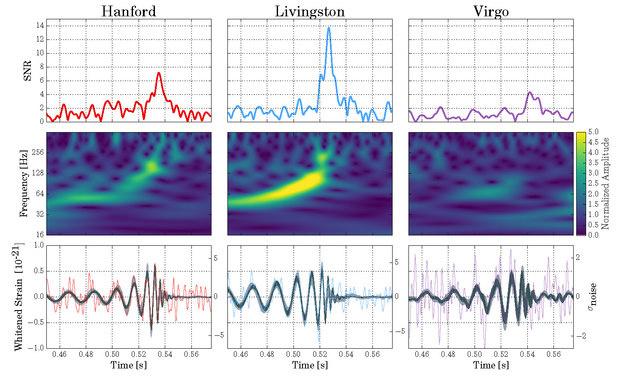
\includegraphics[width=0.8\linewidth]{images/GW.jpg}
        \caption{Immagine copertina}
    \end{figure}
    % 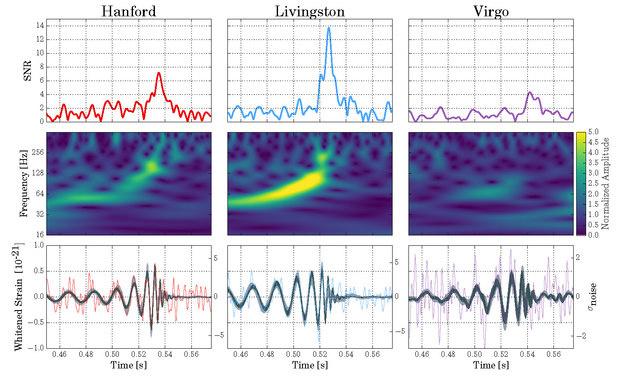
\includegraphics[width=0.8\textwidth]{images/GW.jpg} 
    
    \vfill
    \vspace*{1cm}
    
\end{titlepage}

\newpage

\tableofcontents
\newpage



\cleardoublepage 
\addtocontents{toc}{\bigskip\protect\textbf{\Large Approssimazione Numerica}\par\smallskip}
\addtocontents{toc}{\protect\setcounter{tocdepth}{-2}} 
\part{\Huge Approssimazione Numerica}
\addtocontents{toc}{\protect\setcounter{tocdepth}{2}} 

\section{Esercizio 1.2.1}
\label{sec: basilea}

\subsection{Problem Statement}
Considera la seguente somma

\[
\sum_{n=1}^{\infty} \frac{1}{n^2} = \frac{\pi^2}{6} = \lim_{N \to \infty} S(N) \quad \text{con} \quad S(N) = \sum_{n=1}^{N} \frac{1}{n^2}
\]


\begin{enumerate}
    \item calcolare la somma in precisione singola usando l'ordinamento normale, ovvero iniziando la sommatoria da $n = 1$, poi $2, \dots$ ($n = 1, 2, \dots N$)
    \item calcolare la somma in precisione singola usando l'ordinamento inverso, ovvero iniziando la sommatoria da $n = N$, poi $n = N - 1 \dots$ ($n = N, \dots 2, 1$)
    \item studiare la convergenza di entrambi i metodi in funzione di $N$, graficando $|S(N) - \pi^2/6|$
    \item ripetere i punti 1, 2 e 3 in precisione doppia
\end{enumerate}

\subsection{Premessa Teorica}
Le variabili rappresentate in precisione singola (32 bit) riservano 23 bit alla mantissa, garantendo circa 7 cifre decimali significative. In precisione doppia (64 bit) si hanno invece circa 15-16 cifre significative. Al limite della rappresentazione numerica corrisponde l'errore di arrotondamento (\textit{round-off error}): le operazioni eseguite dal calcolatore conservano questo errore, che viene propagato e influenza la correttezza del risultato.

Il problema richiede di osservare come agiscono gli errori di arrotondamento in funzione della precisione (32-bit, 64-bit). Si propone di risolvere numericamente il calcolo di $S(N)$; il confronto con il valore analitico permette di calcolare l'errore assoluto come:
\[
    \sigma = |S(N) - \pi^2/6|
\]

\subsection{Metodi Numerici e Algoritmi}
È nostro interesse studiare l'effetto dell'arrotondamento al variare di $N$. Ogni termine $\frac{1}{n^2}$ viene valutato imponendo che numeratore e denominatore siano rappresentati nella precisione scelta.

Nella rappresentazione \textit{floating point}, l'operazione di somma dipende dall'ordine di grandezza degli addendi. Quando si sommano numeri molto diversi, il calcolatore deve allineare le mantisse traslando quella del numero più piccolo; se la differenza di ordini di grandezza supera la capacità della mantissa, il contributo del numero minore viene perso.

\noindent L'ordinamento sequenziale con cui procede la somma può essere quindi non indifferente per gli effetti dell'errore di \textit{round-off}, il limite alla precisione è dettato principalmente dalla \textit{machine precision} ($\epsilon_{single} \approx 1.2 \times 10^{-7}, \epsilon_{double} \approx 2.2 \times 10^{-16}$)
\begin{enumerate}

    \item Per l'ordinamento normale (crescente):
    $$
    \sum_{n=1}^N \frac{1}{n^2} = \frac{1}{1^2} + \frac{1}{2^2} + \dots + \frac{1}{N^2}
    $$
    la somma parziale $S(n)$ cresce rapidamente stabilizzandosi vicino a $1.645$. Per $n$ grande, il termine $\frac{1}{n^2}$ diventa trascurabile rispetto a $S(n)$, portando alla perdita di informazione. Esiste un valore di $n$ oltre il quale la somma non aumenta più.

    \item Nell'ordinamento inverso (decrescente), sommiamo prima i termini piccoli tra loro. Questi accumulano una somma parziale che cresce gradualmente, permettendo di conservare cifre significative che andrebbero perse se sommate singolarmente a un valore già grande, risultando in un metodo più preciso per il calcolo della somma (nel confronto per $N$ grande.
\end{enumerate}

\subsection{Risultati e Discussione}
I risultati ottenuti confermano le previsioni teoriche. inoltre l'andamento dell'errore evidenzia due soglie critiche di $N$, dettate dalla precisione di macchina $\epsilon$, oltre le quali il comportamento numerico diverge sensibilmente dal modello analitico.

\subsubsection{$\Tilde{N}_R$}
\noindent In figura \ref{fig: 1 - single precision}, è possibile osservare indicato $\Tilde{N}_R = 1/\epsilon \approx10^7$: questo dà indicazione della correlazione con il punto dal quale la precisione dell'errore assoluto smette di diminuire in maniera proporzionale a N e diventa oscillante: se in particolare scelgo $N > 1/\epsilon \implies \frac{1}{N^2} < \epsilon^2$, quindi completamente invisibile per la precisione singola $\epsilon$. I primi termini della serie non influiranno quindi con un contributo affidabile, ma piuttosto con del rumore numerico che darà il comportamento oscillante.
\footnote{In precisione doppia, questo limite si attesterebbe a $N_R \approx 10^{14}$, un valore computazionalmente proibitivo per questa simulazione.}

\subsubsection{$\Tilde{N}_N$}
\noindent Nell'ordinamento normale, la somma parziale $S(N)$ tende rapidamente al valore asintotico $S \approx 1.645$. Un nuovo termine $1/n^2$ viene ignorato dal calcolatore quando il suo rapporto rispetto alla somma parziale scende sotto la soglia della precisione di macchina:$$    \frac{1/n^2}{S(n)} < \epsilon \implies \frac{1}{n^2} \lesssim 1.645 \cdot \epsilon$$

\noindent Approssimando $S(n) \approx 1$, definiamo $\Tilde{N}_N = 1/\sqrt{\epsilon}$ come il valore di saturazione. Oltre questo limite, ogni ulteriore termine è troppo piccolo per modificare la mantissa della somma già accumulata; l'errore $\sigma(N)$ smette quindi di decrescere e rimane costante (plateau visibile nei grafici).
\[
    \epsilon \ge \frac{1}{n^2} \implies n \ge \frac{1}{\sqrt{\epsilon}}= \Tilde{N}_N \\
\]
\[
    \implies S(n) = S(\Tilde{N}_N) \\
\]
\[
    \implies \sigma(n) = \sigma(\Tilde{N}_N)
\]
\smallskip



\begin{figure} [H]
    \centering
    
\includegraphics[width=0.7\linewidth]{images/2/SinglePrec.png}
    \caption{Andamento dell'errore assoluto $\sigma(N) = |S(N) - \pi^2 / 6|$ usando lo standard a precisione singola, 32-Bit}
    \label{fig: 1 - single precision}
\end{figure}

\begin{figure} [H]
    \centering
    
\includegraphics[width=0.7\linewidth]{images/2/DoublePrec.png}
    \caption{Andamento dell'errore assoluto $\sigma(N) = |S(N) - \pi^2 / 6|$ usando lo standard a precisione doppia, 64-Bit}
    \label{fig: 2 - double precision}
\end{figure}


\newpage









\cleardoublepage 
\addtocontents{toc}{\bigskip\protect\textbf{\Large Matrici e Sistemi Lineari}\par\smallskip}    

\addtocontents{toc}{\protect\setcounter{tocdepth}{-2}} 
\part{\Huge Matrici e Sistemi Lineari} \label{Cap: Matrici e Sistemi Lineari}
\addtocontents{toc}{\protect\setcounter{tocdepth}{2}} 


\section{Esercizio 2.1.1}

\subsection{Problem Statement}
\begin{enumerate}
    \item \textbf{Scrivere una funzione} che accetti una matrice triangolare superiore e implementi la backward substitution. Testarla sul sistema lineare $U\mathbf{x} = \mathbf{b}$ con
    \[
        U = \begin{pmatrix} 2 & 1 & 1 \\ 0 & 1 & -2 \\ 0 & 0 & 1 \end{pmatrix}, \quad \mathbf{b} = \begin{pmatrix} 1 \\ -1 \\ 4 \end{pmatrix}
    \]
    e verificare che la soluzione sia corretta.

    \item \textbf{Scrivere una funzione separata} che esegua la Gauss elimination e combinarla con la Backward substitution per risolvere il sistema
    \[
        \begin{pmatrix} 2 & 1 & 1 \\ 1 & 1 & -2 \\ 1 & 2 & 1 \end{pmatrix} \begin{pmatrix} x_0 \\ x_1 \\ x_2 \end{pmatrix} = \begin{pmatrix} 8 \\ -2 \\ 2 \end{pmatrix}
    \]
    Verificare la soluzione. 

    \item \textbf{Utilizzando i programmi precedenti}, aggiungere una funzione che stampi anche l'inversa esplicita di una matrice. Testarla sulla matrice sopra indicata e verificare il risultato.

    \item \textbf{Adattare i programmi precedenti} per includere il partial pivoting e risolvere i seguenti sistemi. Verificare che senza partial pivoting il programma fallisca, poiché in qualche passaggio intermedio appare $A_{jj} = 0$ per la matrice
    \[
        \begin{pmatrix} 2 & 1 & 1 \\ 2 & 1 & -4 \\ 1 & 2 & 1 \end{pmatrix} \begin{pmatrix} x_0 \\ x_1 \\ x_2 \end{pmatrix} = \begin{pmatrix} 8 \\ -2 \\ 2 \end{pmatrix}
    \]

    \item \textbf{Studiare la soluzione} del problema
    \[
        \begin{pmatrix} 10^{-20} & -1 \\ 1 & 1 \end{pmatrix} \begin{pmatrix} x_0 \\ x_1 \end{pmatrix} = \begin{pmatrix} 1 \\ 2 \end{pmatrix}
    \]
    con e senza pivoting. In questo caso il sistema non è mal condizionato (ovvero non genera infiniti), ma produce un risultato errato. Spiegare l'origine dell'errore e perché il pivoting lo risolve.
\end{enumerate}

\subsection{Premessa Teorica}
Lo scopo dell'esercizio è quello di mettere in luce il più semplice dei metodi numerici per la risoluzione di sistemi lineari di equazioni, sfruttando il formalismo matriciale, risolvendo quindi:
$$
Ax=b
$$
$A$ matrice (quadrata) dei coefficienti, $x$ vettore delle soluzioni (da determinare), $b$ vettore dei termini noti
\subsection{Metodi Numerici e Algoritmi}
\subsubsection{Backward/Forward substitution} \label{sec: Back-Forw Subst}
L'algoritmo fondamentale che usiamo è quello di \textit{Backward/Forward substitution}, cioè che risolve sistemi lineari costruiti da una matrice dei coefficienti che è triangolare superiore/inferiore. Il termine dell'ultima/prima riga è determinabile direttamente, risolvendo $x_i = \frac{b_i}{L_{ii}}$, poi si procede risolvendo per ogni riga in maniera sequenziale e determinando l'intero vettore $x$.\\Per la \textit{Backward} la formula generale è:
$$
x_i = \left( b_i - \sum_{j=i+1}^{n-1} U_{ij}x_j \right) \frac{1}{U_{ii}} \quad i = n-1, \dots , 0
$$
per la \textit{Forward}:
$$
x_i = \left( b_i - \sum_{j=0}^{i-1} L_{ij}x_j \right) \frac{1}{L_{ii}} \quad i = 0, \dots, n-1
$$

\subsubsection{Gaussian Elimination}
Si può generalizzare la soluzione di un sistema lineare per una matrice $A$ quadrata generica. Per fare ciò usiamo un algoritmo che permetta di riportare $A$ nella forma di $U$ (triangolare superiore), in maniera da poter risolvere usando la \textit{Backward substitution}. È possibile sviluppare l'algoritmo partendo da semplici operazioni sulle matrici, nel corso delle quali si sceglie una riga di riferimento (pivot row) e la si usa per annullare tutti gli elementi delle righe al di sotto di questa. Ci si sposta quindi nella riga successiva, fino a che non si rende $A$ una triangolare superiore. Si possono quindi combinare \textit{Gaussian elimination} (GE) e \textit{Backward substitution} (BS) in una unica funzione.

\subsubsection{Partial Pivoting}
In caso di matrici mal condizionate, può accadere che la scelta del \textit{pivot} non sia irrilevante: in questi casi, l'operazione di \textit{Partial pivoting} (PP) permette di stabilizzare il processo, scambiando la riga pivot \textit{p}, nella colonna \textit{j}, con la riga \textit{i} con l'elemento $A_{ij}$ massimo rispetto a quelli nella colonna.

\subsubsection{Inversa di una Matrice} \label{sec: inverse of a matrix}
Combinando gli algoritmi sopra definiti è possibile anche determinarne uno per trovare l'inverso di una matrice generica $A$. Data la generica $A\in \mathbb{C}^{n\times n}$ e $\mathbb{I}_n$, matrice identità:
$$
A^{-1} = (x_0,\ x_1,\ \dots\ , x_{n-1})
$$

\noindent cioè la colonna i-esima della matrice $A^{-1}$ sarà data dalla soluzione al sistema 
$$
A\ x_i = \mathbb{I}_i  
$$
dove $\mathbb{I}_i$ è la colonna i-esima della matrice identità.

\newpage

\subsection{Risultati e Discussione}
Di seguito i risultati e le soluzioni ai problemi presentati nella consegna:
\begin{multicols}{2} % Inizio delle due colonne
\begin{enumerate}[series=miolista]

   \item Risoluzione del sistema $Ux = b$ tramite BS:
    \begin{elegantcode}
U =
 [[ 2.  1.  1.]
 [ 0.  1. -2.]
 [ 0.  0.  1.]]
b = [ 1. -1.  4.]

Solution found:
x = [-5.  7.  4.]
    \end{elegantcode}

\item Risoluzione del sistema generico tramite GE e BS; usiamo una versione di GE "ingenua":

\begin{elegantcode} 
A =
 [[ 2.  1.  1.]
 [ 1.  1. -2.]
 [ 1.  2.  1.]]
b = [ 8. -2.  2.] 

x = [ 4. -2.  2.]
    \end{elegantcode}

    \item L'inversa può essere determinata come definito nell'algoritmo in \ref{sec: inverse of a matrix}:
    \begin{elegantcode} 
A =
 [[ 2.  1.  1.]
 [ 1.  1. -2.]
 [ 1.  2.  1.]] 

Solution found:
A^-1 =
 [[ 0.625  0.125 -0.375]
 [-0.375  0.125  0.625]
 [ 0.125 -0.375  0.125]]
    \end{elegantcode}

    \item La prova del fallimento dell'algoritmo "ingenuo" determina la necessaria modifica a GE per introdurre PP e generalizzare il suo utilizzo:

    \begin{elegantcode}[title=Uso di \textit{BackGauss\_dumb()} e problemi relativi agli infiniti]
An error occured!!: Algorithm fails!
b != U * x 
RuntimeWarning: divide by zero encountered in scalar divide
  c = A[i,j] / A[j,j]
RuntimeWarning: invalid value encountered in multiply
  A[i,:] -= c * A[j,:]
RuntimeWarning: invalid value encountered in scalar divide
  x_i = (b[i] - np.dot(U[i, i+1:], np_xi[i+1:])) / U[i, i]
    \end{elegantcode}

    \begin{elegantcode}[title=Uso di \textit{BackGauss()} per trovare la soluzione del problema (implementazione di PP)]
A =
 [[ 2.  1.  1.]
 [ 2.  1. -4.]
 [ 1.  2.  1.]]
b = [ 8. -2.  2.] 

Solution:
x = [ 4. -2.  2.]
    \end{elegantcode}
\end{enumerate}
\end{multicols}

\begin{enumerate}[resume=miolista]
    \item Il pivoting garantisce stabilità anche con matrici non mal condizionate, evitando errori di assorbimento in virgola mobile. Analiticamente:
    \[
    \begin{pmatrix} 10^{-20} & -1 \\ 1 & 1 \end{pmatrix}
    \begin{pmatrix} x_0 \\ x_1 \end{pmatrix} =
    \begin{pmatrix} 1 \\ 2 \end{pmatrix} \implies
    \begin{cases} x_0 = 3 \\ x_1 = -1 \end{cases}
    \]

    Nell'esecuzione del programma senza pivoting il problema si incontra nel momento in cui, tenendo come pivot la prima riga, svolgiamo:
    $$c =\frac{A_{10}}{A_{00}}=10^{20} \implies
    \begin{cases}
        A_{10} = 0 \\
        A_{11} = 1+10^{20}\\
        b_1 = 2-10^{20}
    \end{cases}    
    $$    
    Dall'analisi dei risultati emerge chiaramente la criticità intrinseca nelle operazioni effettuate. Nello specifico, il calcolo di espressioni quali $1+10^{20}$ o $2-10^{20}$ evidenzia i limiti strutturali della rappresentazione numerica finita.
    
    L'elaboratore opera in precisione doppia, uno standard che garantisce una risoluzione di circa 15-16 cifre significative. Quando si confrontano operandi che differiscono per 20 ordini di grandezza, il valore minore scende al di sotto della precisione di macchina ($\epsilon_m$). 
    
    Di conseguenza, durante l'allineamento delle mantisse, il numero più piccolo viene "assorbito" da quello maggiore, rendendo l'operatore insensibile alla variazione. Si verifica pertanto il fenomeno dell'errore di arrotondamento per cui:
    
    $$
    \begin{cases}
        A_{11} = 1+10^{20} \approx 10^{20}\\
        b_1 = 2-10^{20} \approx -10^{20}
    \end{cases}    
    $$    
    
    $$
        \begin{pmatrix}
            10^{-20} & -1 \\
            0 & 10^{20}
        \end{pmatrix}
        \begin{pmatrix}
            x_0 \\x_1
        \end{pmatrix} =
        \begin{pmatrix}
            1 \\ -10^{20}
        \end{pmatrix}
    $$
    $$
    \implies \begin{cases}
        x_1 = \frac{-10^{20}}{10^{20}} = -1 \\
        x_0 = \frac{1 - x_1}{10^{-20}} = 0 
    \end{cases}
    $$
    cioè un risultato inesatto! Il metodo senza PP ci conduce a sbagliare nettamente la risposta al problema.
        
    \noindent L'output generato dall'esecuzione degli script conferma l'analisi precedente:\\
    
    \begin{elegantcode}
% Senza Pivoting (Errore)
x_dumb = [ 0. -1.]
% Con PP (Corretto)
x_true = [ 3. -1.]
    \end{elegantcode}
    
    \noindent L'esperimento dimostra che una matrice non mal condizionata (il cui determinante è significativamente diverso da zero) può comunque portare al fallimento dell'algoritmo di Gauss se non si adotta il pivoting parziale.
    
\end{enumerate}
\newpage





\section{Esercizio 2.2.1}
\label{sec: poisson res}
\subsection{Problem Statement}
Scrivere un programma che accetti una matrice $A$, verifichi che sia simmetrica (se reale) e restituisca quindi il fattore di Cholesky $L$.

\begin{enumerate}
    \item Testare il programma sulla matrice
    \[
    \begin{pmatrix}
    4 & 12 & -16 \\
    12 & 37 & -43 \\
    -16 & -43 & 98
    \end{pmatrix}
    \]
    e verificare la correttezza del risultato.
    
    \item Scrivere un risolutore che combini la fattorizzazione di Cholesky con le \textit{forward} e \textit{backward substitution}.
    
    \item Calcolare la matrice laplaciana $K$ e il vettore $b$ utilizzando
    \begin{itemize}
        \item $4\pi\varepsilon_0 = 1.0$
        \item $L = 1.0$
        \item $N = 50$
        \item densità di carica distribuita gaussianamente $\rho(x) = e^{-R(x-0.5)^2}$
    \end{itemize}
    
    Risolvere il sistema lineare per i casi $R = 100$ e $R = 10$ utilizzando il risolutore basato sulla decomposizione di Cholesky.
\end{enumerate}


\subsection{Premessa Teorica}
Una matrice non singolare $A$ può essere espressa come prodotto di due matrici triangolari, inferiore e superiore, cioè:
\[
A = LU
\]
dove questa cosiddetta \textit{decomposizione LU} non è unica: è imponendo alcune condizioni che possiamo determinare univocamente le due, quindi possiamo risolvere il sistema generico 
\[
Ax = b
\]
eseguendo una combinazione di BS e FS. \textit{Il teorema di decomposizione di Cholesky} afferma inoltre che per una qualsiasi matrice hermitiana definita positiva esiste ed è unica la matrice $L$ (Fattore di Cholesky) t.c.:
\[
A = LL^\dagger
\]

\subsection{Metodi Numerici e Algoritmi}
Analizzando la definizione di $A=LL^\dagger$, esprimendo esplicitamente il prodotto delle due matrici a destra, si può evidenziare come sia possibile determinare $L$ con una funzione ricorsiva partendo solo da $A$, iterando sulle sue righe e colonne. Ciò permette di risolvere il sistema lineare, in particolare:
\[
Ax = LL^\dagger x = Ly = b\ , \quad L^\dagger x = y
\]
\[
\begin{cases}
    Ly = b \quad (\text{FS, ricavo $y$})\\
    L^\dagger x = y \quad (\text{BS, ricavo $x$})
\end{cases}
\]
al termine della seconda interazione ho quindi determinato univocamente le soluzioni del sistema lineare definito inizialmente su $A$, matrice dei coefficienti.
\\
Se dal punto di vista del costo computazionale questo approccio presenta un leggero guadagno rispetto a quello della LU (entrambi proporzionali a $n^3$) la vera grande differnza sta nella stabilità dell'algoritmo della \textit{decomposizione di Cholesky}: di fronte ad una matrice $A$ mal condizionata, quindi con un $\kappa(A)$ grande, $L$ è in generale proporzionale al \textit{condition number}, ma il prodotto $LL^\dagger$ presenta molte semplificazioni che determinano:
\[
\Tilde{L}\Tilde{L}^\dagger = A + \delta A
\]
dove $\Tilde{L}$ è il \textit{Cholesky factor} di $A$ più una sua piccola variazione. La variazione su $A$ può modificare anche significativamente $L$, ma il prodotto con la sua aggiunta differisce dal risultato imperturbato di una piccola quantità, proprio grazie alle semplificazioni nel calcolo del prodotto che bilanciano l'operazione.

\subsection{Risultati e Discussione}
\begin{enumerate}
   \item Test di funzionamento della funzione per $L$
    \begin{elegantcode} 
A:
 [[  4.  12. -16.]
 [ 12.  37. -43.]
 [-16. -43.  98.]]

Cholesky factor (L):
 [[ 2.  0.  0.]
 [ 6.  1.  0.]
 [-8.  5.  3.]]
    \end{elegantcode}
    Il test di correttezza del risultato avviene confrontando $LL^\dagger$ con $A$ e aspettandosi una differenza confrontabile con zero tra le due matrici.

    \item Il problema richiede la risoluzione dell'\textit{Equazione di Poisson} (\ref{eq: Poisson}) per via numerica: questo è un caso ottimo per sfruttare le potenzialità dell'algoritmo che abbiamo mostrato, in particolare perché la soluzione di
    \begin{equation} \label{eq: Poisson}
        \nabla^2 \phi\text{(r)} = -\frac{\rho\text{(r)}}{4\pi\varepsilon_0}
    \end{equation}
    può essere ricavata discretizzando il dominio e approssimando la derivata seconda con il metodo delle differenze finite
    \footnote{Secondo le differenze finite:
    $\frac{d^2\phi}{dx^2} \approx \frac{\phi_{i-1} - 2\phi_i + \phi_{i+1}}{a^2}$
    }
    . Inoltre imponiamo le \textit{NU} ($4\pi \varepsilon_0 = 1$) per praticità; risulta quindi
    $$
    -\phi_{i-1} + 2\phi_i - \phi_{i+1} = a^2\rho_i
    $$
    Imponendo le condizioni al contorno $\phi(0)=\phi(L)=0$ e assorbendo $a^2$ nella definizione di $\rho$ ($\rho \leftarrow{} a^2 \rho$) otteniamo un sistema di equazioni lineari in forma matriciale:
    
    \begin{equation} \label{eq: eq lin poisson}    
    K\phi = b
    \end{equation}

    $$
    K = \begin{pmatrix}
        2 & -1 & 0 & \dots & 0 \\
        -1 & 2 & -1 & \dots & 0 \\
        0 & -1 & 2 & \dots & 0 \\
        \vdots &&& \dots & -1 \\
        0 & \dots & \dots & -1 & 2 \\
    \end{pmatrix},\ \ \ b = \begin{pmatrix}
        \rho_1 \\ \rho_2 \\ \vdots \\ \rho_N
    \end{pmatrix}    
    $$
    
    Dove $K$ è la rappresentazione matriciale dell'operatore laplaciano e $b$ è il vettore discretizzato della densità di carica. Saremo agili nel risolvere il sistema lineare (\ref{eq: eq lin poisson}) con i metodi sviluppati finora; in particolare useremo la decomposizione di Cholesky.

    Definendo una distribuzione di carica gaussiana intorno all'origine, come da consegna:
    \[
    \rho(x) = e^{-R(x-0.5)^2} \text{, \quad}\  x \in [0, L]\ \xrightarrow{\text{norm.}}x/L \in [0, 1] 
    \]
    È possibile osservare la soluzione dell'equazione di Poisson nella figura qui sotto; al variare del parametro $R$ il profilo di $\phi$, potenziale generato dalla carica $\rho$.
    \begin{center}
        
\includegraphics[width=0.7\linewidth]{images/4/poiss_sol.png}
        \captionof{figure}{Soluzione dell'equazione di Poisson $\phi$ per $R=100$ e $R=10$} 
        \label{fig: poiss_label}
    \end{center}
\end{enumerate}

\newpage









\cleardoublepage 
\addtocontents{toc}{\bigskip\protect\textbf{\Large Ricerca degli Autovalori}\par\smallskip}
\addtocontents{toc}{\protect\setcounter{tocdepth}{-2}} 
\part{\Huge Ricerca degli Autovalori}
\addtocontents{toc}{\protect\setcounter{tocdepth}{2}} 



\section{Esercizio 3.1.1}
\subsection{Problem Statement}

Considera la matrice
\[
A = \begin{pmatrix}
4 & -i & 2 \\
i & 2 & 2 + 7i \\
2 & 2 - 7i & -2
\end{pmatrix}
\]

\begin{enumerate}
    \item Calcola l'autovalore massimo e il corrispondente autovettore utilizzando il \textit{Power Method}. Introduci un criterio di arresto basato su una data tolleranza sull'autovalore, ad esempio $10^{-6}$, o basato su un numero massimo di iterazioni. Verifica la correttezza dell'algoritmo.
    
    \item Calcola l'autovalore minimo con il \textit{Inverse Power Method} utilizzando il risolutore QR sviluppato negli esercizi precedenti.
    
    \item Studia numericamente la convergenza degli algoritmi. Definisci $\lambda_1^n$ come l'autovalore massimo ottenuto dal \textit{Power Method} dopo $n$ iterazioni e $\lambda_3^n$ come l'autovalore minimo ottenuto dall'\textit{Inverse Power Method}. Successivamente, rappresenta graficamente $|\lambda_1^n / \lambda_1 - 1|$ e $|\lambda_3^n / \lambda_3 - 1|$ in funzione delle iterazioni.
\end{enumerate}

\subsection{Premessa Teorica}
Il \textit{Power Method} (\textit{PM}) è uno degli algoritmi più semplici per estrarre gli autovalori di una generica matrice $A \in \mathbb{C}^{N \times N}$ diagonalizzabile e con un autovalore dominante in modulo, in particolare, il metodo restituisce una stima dell'autovalore di modulo maggiore. È possibile definire un \textit{Inverse Power Method} (\textit{IPM}) che determini l'autovalore minimo della matrice. Questi vengono definiti algoritmi iterativi, cioè che determinano il risultato con uno specifico grado di precisione, ma non convergono in un numero finito di passaggi al valore vero. Nel corso della discussione dei metodi presenentiamo il caso di matrice reale per semplicità: il passaggio ad una complessa richiede di sostituire $A^T \longrightarrow A^\dagger$.

\subsection{Metodi Numerici e Algoritmi}
\subsubsection{Power Method}
Data $A^{N\times N}$ e scegliendo un generico vettore di partenza $\boldsymbol{x_0}$, possiamo definire:
\[
\boldsymbol{y}(n) = A^n \boldsymbol x_0 = \dots = \lambda_1^n \left[ c_1 \boldsymbol{v}_1 + \sum_{i=2}^{N} c_i \left( \frac{\lambda_i}{\lambda_1} \right)^n \boldsymbol{v}_i \right], \quad \quad \left| \frac{\lambda_i}{\lambda_1} \right| < 1
\]
quindi, grazie all'ultima riscrittura, prendendo il limite per $n \xrightarrow{} \infty$, cioè per un grande numero di iterazioni dell'algoritmo:
\begin{equation} \label{eq: Direct Method autovett}
\lim_{n \xrightarrow{}\infty} \boldsymbol{y}(n) = c_1 \lambda_1^n \boldsymbol{v}_1
\end{equation}
L'ultimo risultato ci porta a determinare univocamente, a meno della normalizzazione, l'autovettore associato a $\lambda_1$. La soluzione è non banale se e solo se il vettore iniziale $\boldsymbol x_0$ non è ortogonale
\footnote{
Ci occupiamo di questa eventualità semplicemente definenedo il vettore $\boldsymbol x_0$ con direzione casuale.
}
a $\boldsymbol{v}_1$, poichè quello che l'algoritmo fa è applicare la matrice al vettore generico, ridirezionandolo e riscalandolo:
\begin{enumerate}
    \item Con la normalizzazione ad ogni step eliminiamo il \textit{rescaling} ($y \longrightarrow \frac{y}{||y||}$).
    \item Iterando per un numero di volte sufficientemente grande vediamo che il contributo principale è quello dell'autovalore maggiore, quindi ci aspettiamo che il vettore finale sia sovrapponibile all'autovettore associato a $\lambda_1$ (cfr. Eq.~\eqref{eq: Direct Method autovett}).
\end{enumerate}
Alla definizione dell'autovettore possiamo infine discutere quella dell'autovalore, usando il "Coefficiente di Rayleigh" come segue:
\begin{equation} \label{eq: Rayleigh Coeff}
\lim_{n\to\infty} \lambda_1^{(n)} = \lim_{n\to\infty} \frac{\boldsymbol{y}(n)^T A \boldsymbol{y}(n)}{\boldsymbol{y}(n)^T \boldsymbol{y}(n)} = \lambda_1
\end{equation}

\noindent Per ottimizzare l'algoritmo definiamo $\boldsymbol y = A\boldsymbol x_0$, successivamente calcoliamo per ogni interazione\\ $\boldsymbol y(k+1) = A\boldsymbol y(k)$: quando terminiamo l'algoritmo, dopo un numero $n$ di iterazioni, il valore di $\boldsymbol y(n) = A^n \boldsymbol x_0$.\\

\noindent Si può dimostrare che il \textit{Power Method} così definito ha convergenza lineare.

\subsubsection{Inverse Power method} \label{sec: Inverse Pow mth}
Analizzando la matrice inversa di $A$ possiamo dire che essa avrà gli stessi autovettori dell'originale, ma le corrisponderanno autovalori inversi, cioè:
\[
A\boldsymbol v_1 =\lambda_1 \boldsymbol v_1 \xrightarrow{Inversa} A^{-1}\boldsymbol v_1 = \frac{1}{\lambda_1} \boldsymbol v_1
\]
Questo comporta che l'autovalore più piccolo di A diventa il più grande per la sua inversa, possiamo quindi applicare il \textit{PM} e definire iterativamente
\[
\boldsymbol	y(n+1) = A^{-1}\boldsymbol y(n)
\]
Valutare l'inversa di una matrice generica è un'operazione costosa, è però possibile riscrivere la relazione come segue, evitando di dover invertire:
\[
A\boldsymbol y(n+1) = \boldsymbol y(n)
\]
decidiamo infine di procedere implementando l'utilizzo degli algoritmi di scomposizione, in particolare scegliamo \textit{QR decomposition}: 
\[
A = QR 
\]
\[
\longrightarrow{} QR\boldsymbol y_{n+1} = \boldsymbol y_n
\]
\[
\longrightarrow{}R\boldsymbol y_{n+1} = Q^{-1} \boldsymbol y_n
\]
Ricordando che per le proprietà della decomposizione QR, $Q^TQ = I \longrightarrow{}Q^{-1} = Q^T$ (cioè $Q$ è ortogonale)
\[
R\boldsymbol y_{n+1} = Q^T \boldsymbol y_n
\]
ridefinendo $\boldsymbol{b} = Q^T \boldsymbol y_n$, quello che rimane è un sistema lineare molto facilmente risolvibile, tramite una semplice \textit{Backward Substitution} (cfr Cap. \ref{sec: Back-Forw Subst})
\[
R\boldsymbol y_{n+1} = \boldsymbol{b}
\]
ancora una volta, per un numero grande di iterazioni, $\boldsymbol y_n = \boldsymbol v_N$, dove $\boldsymbol v_N$ è l'autovettore relativo all'autovalore più piccolo.
\subsubsection{Shifting}
Un'estensione di questo algoritmo è possibile considerando lo \textit{shifting}: scegliendo un valore di riferimento si può spostare lo spettro di $A$ di un certo scalare.\\
Se scelto in maniera oculata, questo può essere un grande vantaggio, per esempio possiamo ridefinire la matrice come $A \xrightarrow[]{}A - \alpha I$, spostando tutti gli autovalori da $\lambda \xrightarrow[]{}\lambda - \alpha$: se scegliamo $\alpha$ vicino ad un generico autovalore $\lambda_k$ di tutti gli $N$ della matrice, l'operazione che abbiamo appena definito rende $\lambda_k$ quello in modulo più piccolo, che avrà dopo lo \textit{shifting}, un valore confrontabile con lo zero, risultando, guardando la matrice inversa, in un autovalore grande, che permette ad $A^{-1}$ di trasformare il vettore generico proprio in $\boldsymbol{v}_k$ (normalizzato) con poche interazioni.\\
Per avere una stima di $\lambda_k$ da usare come $\alpha$, ricorriamo al \textit{Rayleigh Quotient}, cioè utilizzando la migliore stima possibile, ad una certa iterazione, dell'autovalore.\\
\noindent Si può dimostrare che il Metodo del Quoziente di Rayleigh ha convergenza cubica (e che costa $O(N^2)$, grazie all'utilizzo della \textit{Backward Substitution} e della \textit{QR decomposition}).


\subsection{Risultati e Discussione} \label{sec: Controllo autovalori}
Procediamo ad analizzare le soluzioni ai problemi proposti nell'esercizio:
\begin{enumerate}
    \item Tramite implementazione del \textit{PM} risolviamo il problema della ricerca dell'autovalore in modulo maggiore:
    \begin{elegantcode}
A =
[[ 4.+0.j -0.-1.j  2.+0.j]
 [ 0.+1.j  2.+0.j  2.+7.j]
 [ 2.+0.j  2.-7.j -2.+0.j]]

eig_val_MAX = (8.451876899596735+8.881784197001252e-16j)
eig_vect = [0.63491092-0.59342626j 1.18122253+0.91110263j 0.95772132-0.73031907j]
    \end{elegantcode}
    Abbiamo definito che l'algoritmo abbia arresto nel momento in cui $|\lambda_{n+1} - \lambda_n| <\varepsilon = 10^{-8}$.\\
    Viene valutata la correttezza dei risultati finali in questo modo:
    \begin{elegantcode}
res = A @ eigVect - eigVal * eigVect
err = np.sqrt(np.sum(np.abs(res)**2))
if err > 1e-8:
    raise ValueError("Eigenpair not accurate")
    \end{elegantcode}
    cioè secondo la definizione di autovalore $A \boldsymbol v =\lambda\boldsymbol v$.
    
    \begin{multicols} {2}
        È interessante osservare come l'errore sull'autovalore calcolato, per ogni iterazione, abbia un decadimento esponenziale. In particolare nella Figura \ref{fig: Plot conv Power Mth} rappresentiamo il caso di due matrici $M \in \mathbb{R}^{3\times 3}\ , K \in \mathbb{C}^{3\times 3}$. Per le considerazioni fatte nei paragrafi precedenti ci aspettiamo, in un eventuale confronto, che il \textit{IPM}, a parità di matrice di test, abbia necessità di meno interazioni per arrivare a convergenza.
        
        \begin{figure}[H]
            \centering
            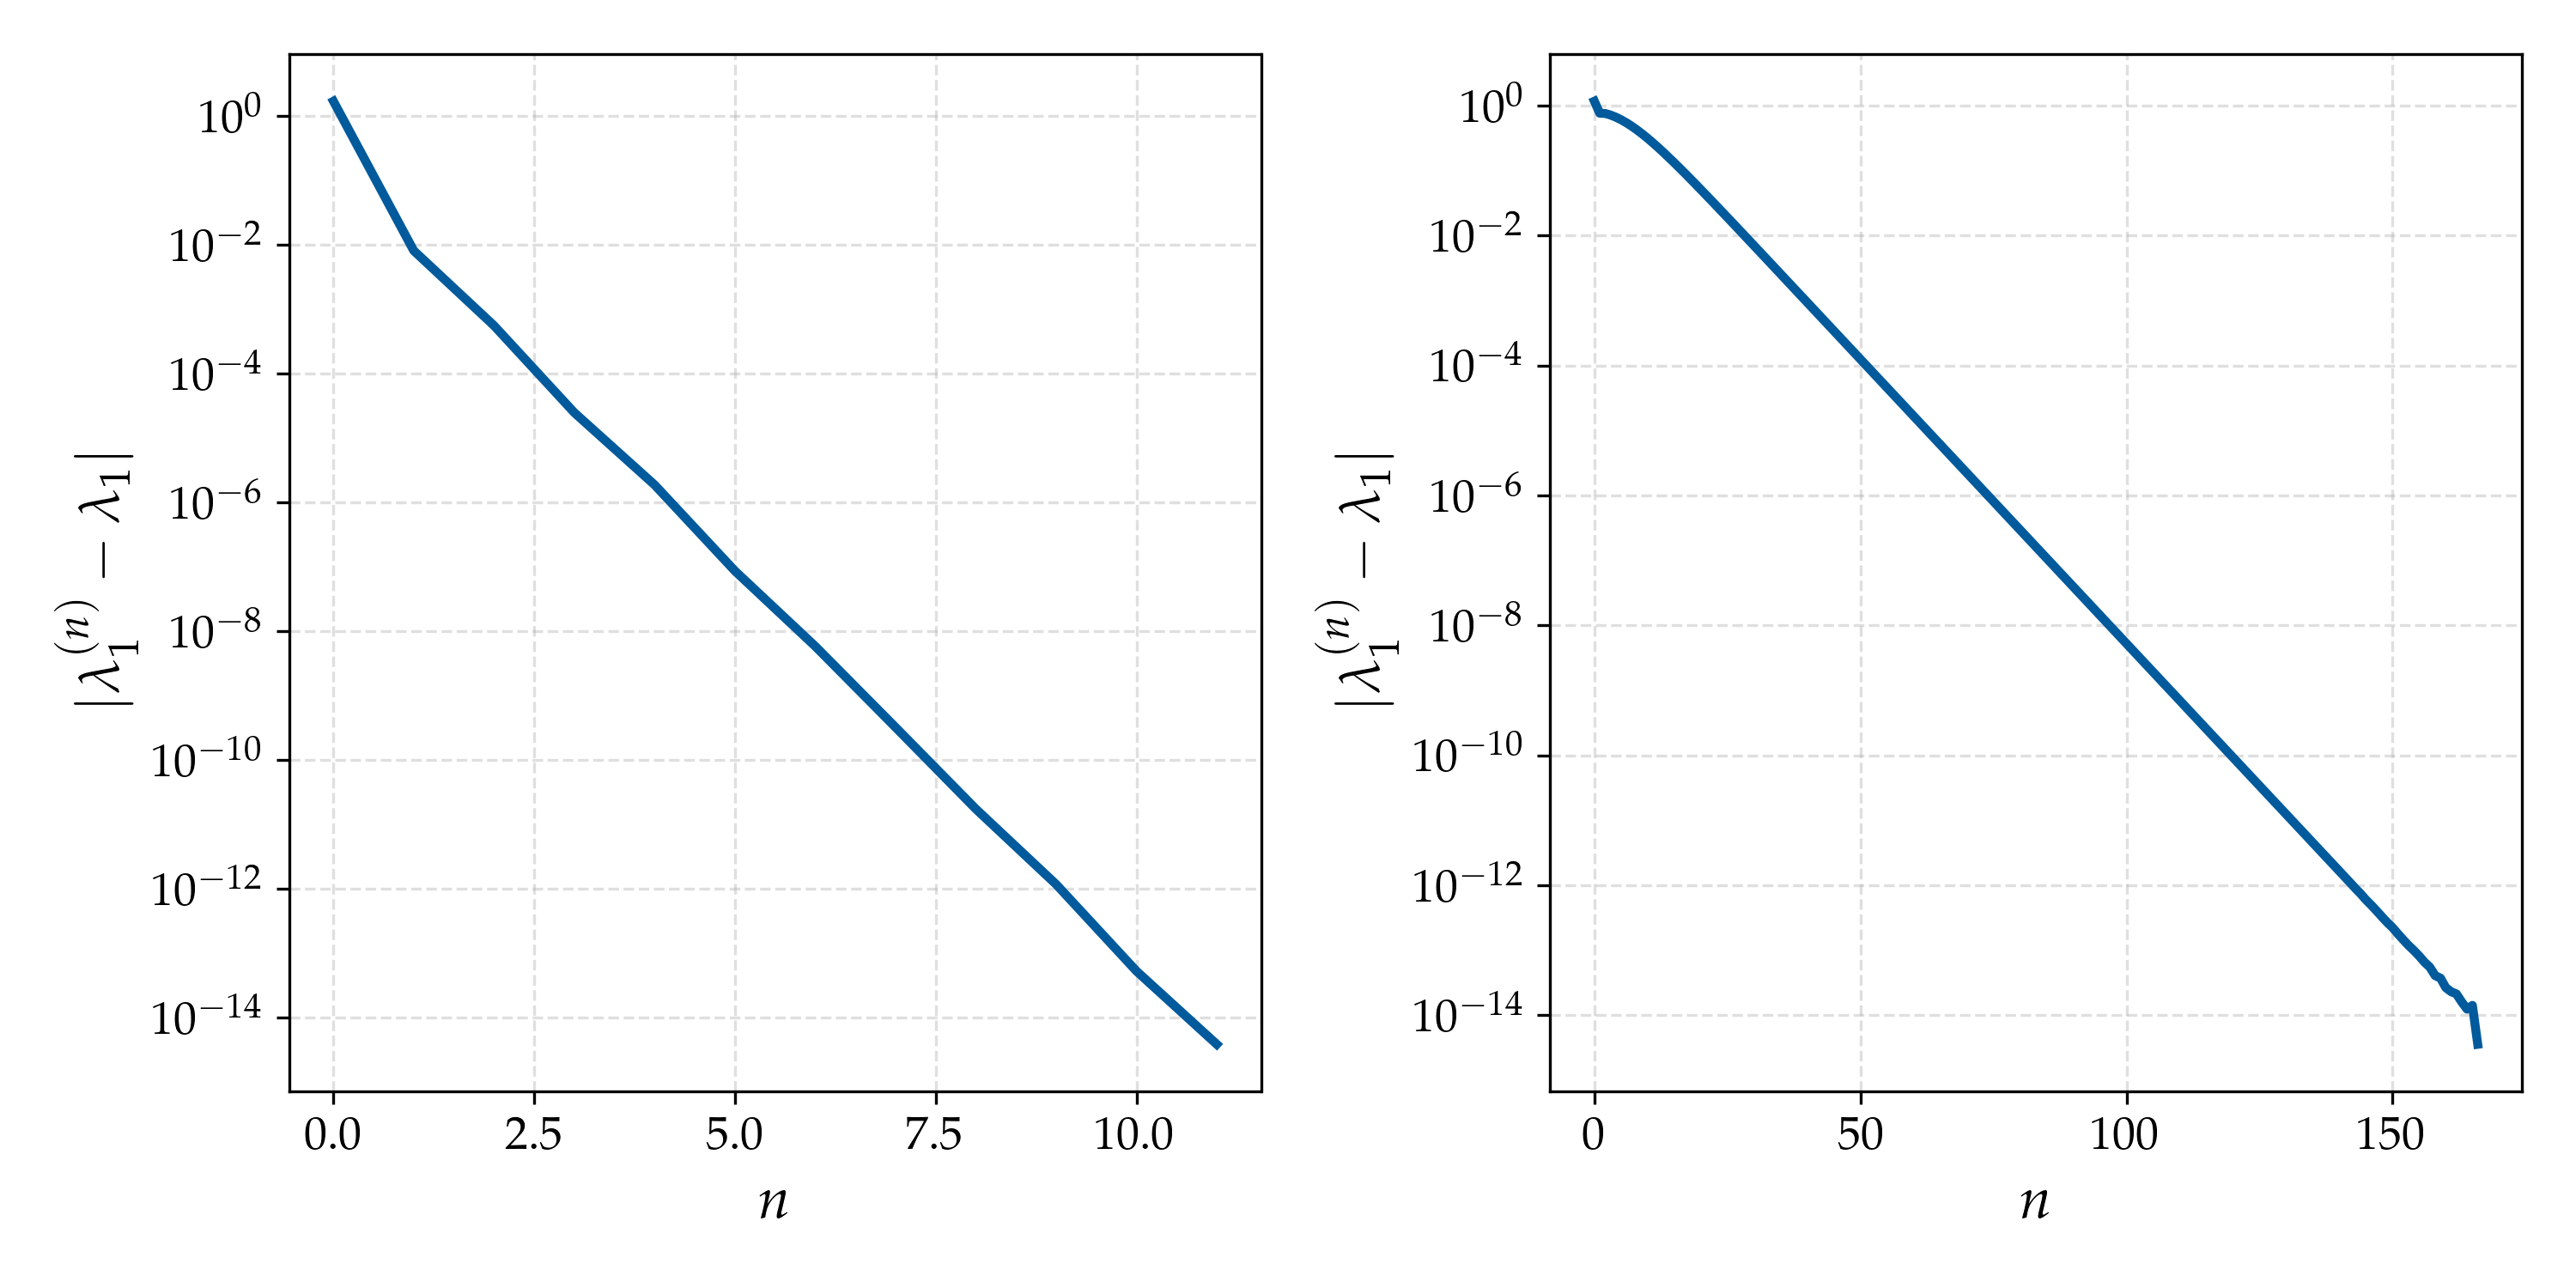
\includegraphics[width=1.1\linewidth]{images/6/plot_powConv.png}
            \caption{Sulla sinistra il caso di $M$, sulla destra $K$. L'andamento della convergenza è lo stesso ma si noti la differenza nel numero di iterazioni necessarie per
            raggiungere la precisione}
            \label{fig: Plot conv Power Mth}
        \end{figure}
    \end{multicols}    

    \item In maniera del tutto simile a quanto fatto in precedenza, e in accordo con ciò che abbiamo descritto nel Cap. \ref{sec: Inverse Pow mth}, risolviamo il problema con questo output:
    \begin{elegantcode}
A =
[[ 4.+0.j -0.-1.j  2.+0.j]
 [ 0.+1.j  2.+0.j  2.+7.j]
 [ 2.+0.j  2.-7.j -2.+0.j]]
 
eig_val_min = (3.1896027470480552-3.51669076861739e-17j)
eig_vect = [ 1.063511 -0.0526563j -0.1124258-0.4313319j -0.2152674-0.0348766j]
    \end{elegantcode}
    
    \item Infine possiamo confrontare i risultati dei due metodi. Gli algoritmi completi sono stati modificati in maniera da restituire la stima dell'autovalore ad ogni step, fino ad un valore fissato di $n=80$ dal quale in poi la precisione dell'\textit{IPM} ha raggiunto la \textit{machine precision} $\varepsilon \approx 10^{-15}$.
    
    
    I valori di confronto per i rapporti ($\lambda_{\text{MAX}}$ e $\lambda_{min}$)sono dati dai punti precedenti dell'esercizio, in cui li abbiamo calcolati esplicitamente. È possibile notare una differenza netta tra la convergenza del primo o del secondo metodo: l'autovalore più piccolo risulta, guardando la matrice inversa, in uno grande, quindi l'effetto dipende dal rapporto tra gli autovalori dell’inversa, cioè $\left|\lambda_{N-1}/\lambda_N\right|$. Ne risulta che l'applicazione della matrice sul vettore random di inizializzazione, ha un effetto più marcato con l'\textit{Inverse}, permettendo una rapida convergenza.

    \begin{figure}[H]
        \centering
        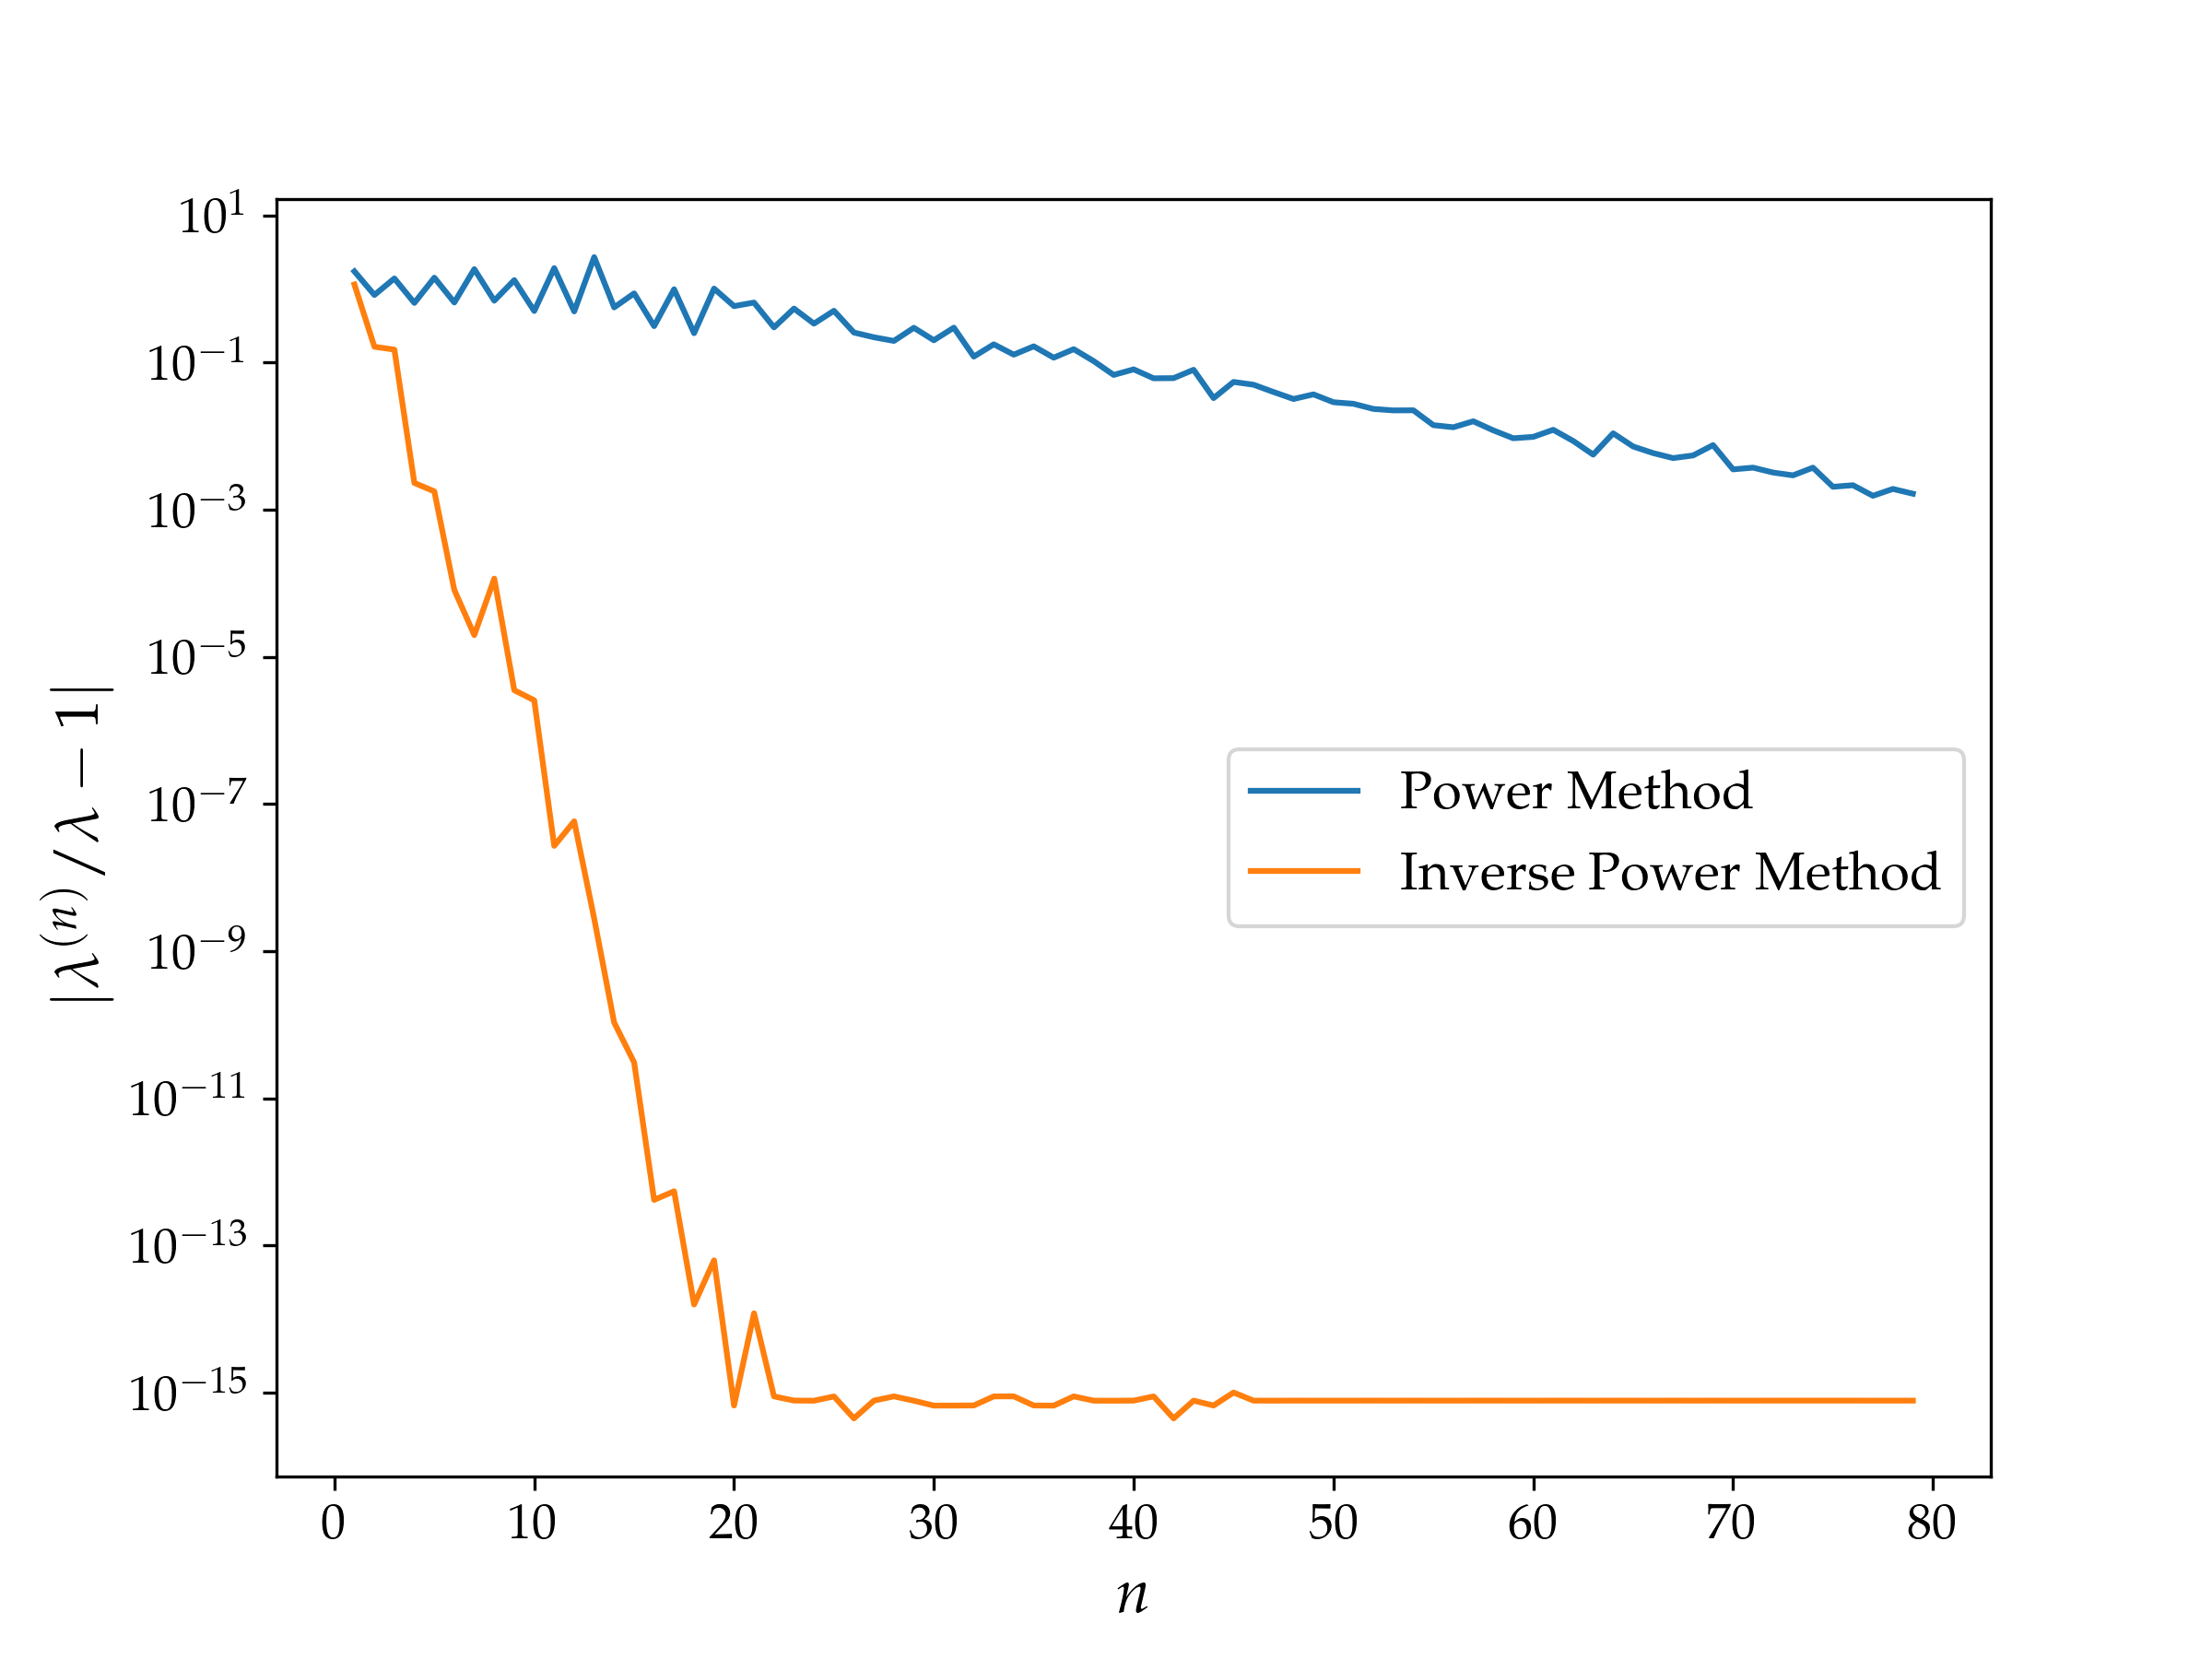
\includegraphics[width=0.7\linewidth]{images/6/pow_vs_inv_convergence.png}
        \caption{Confronto tra il rate di convergenza del \textit{PM} (blu) e quello dell'\textit{IPM} (giallo)}
        \label{fig: Conv Pow vs Inv}
    \end{figure}
\end{enumerate}








\newpage

\section{Esercizio 3.2.1}
\subsection{Problem Statement}
Si implementi una funzione che riceva in ingresso una matrice $A$, una tolleranza $\epsilon$ e un numero massimo di iterazioni $N$. La funzione deve restituire gli autovettori e gli autovalori di $A$ attraverso l'applicazione iterativa della decomposizione $QR$ precedentemente implementata.\\
Poiché si prevede che la matrice risultante $A_\infty$ sia una matrice diagonale (o triangolare superiore a blocchi) contenente gli autovalori lungo la diagonale principale, si definisca un criterio di arresto appropriato. Per testare l'algoritmo, si utilizzi la matrice tridiagonale che rappresenta l'operatore Laplaciano unidimensionale, considerando dimensioni modeste dell'ordine di $O(10)$.\\
Si produca infine un grafico che mostri l'andamento della convergenza per ogni singolo autovalore in funzione del numero di iterazioni.

\subsection{Premessa Teorica}
Una possibilità per lo sviluppo di un algoritmo di estrazione degli autovalori di una matrice sta nei metodi di decomposizione della matrice di test $A$: se è effettivamente possibile implementare un algoritmo che faccia uso della Decomposizione LU, è molto più conveniente lo sviluppo di uno che usi la Decomposizione QR, più stabile e possibile per una qualsiasi matrice generica. Questo rappresenta un metodo di algoritmo iterativo, portandosi dietro tutte le sue potenzialità, ma anche le sue problematiche.

\subsection{Metodi Numerici e Algoritmi}
Si procede definendo iterativamente $A_k$, fissando $A_0 = A$: da qui in poi, potendo decomporre con \textit{QR decomposition}, quindi $A_k = Q_kR_k$, si definisce la matrice al passo $k+1$ come $A_{k+1}=R_kQ_k$. Questa operazione è una trasformazione di similitudine, infatti si può mostrare che $A_{k+1}=Q^\dagger_k A_k Q_k$, e la sua importanza sta nel fatto di conservare lo spettro della matrice originale.\\
Per un numero grande di iterazioni:
\begin{enumerate}
    \item $A_k$ converge verso $A_\infty$, che è la sua diagonalizzata, cioè presenta gli autovalori sulla diagonale e zeri nel resto.
    \item $\prod_{j=0}^k Q_j$, converge a $Q_\infty$, le cui colonne sono gli autovettori che costituiscono una base ortonormale di $A$.
\end{enumerate}
Queste conclusioni sono valide nella maniera qui esposta solo per matrici hermitiane, per una matrice generica $A_\infty$ è triangolare superiore e l'algoritmo si complica. Ci limitiamo quindi a studiare matrici hermitiane, che sono una classe abbastanza rappresentativa per i problemi di fisica che andremo ad analizzare.

\subsection{Risultati e Discussione}
Il test sulla ricerca degli autovalori viene fatto su una matrice $A \in \mathbb{C}^{3 \times 3}$ (hermitiana), definita come segue:
\begin{elegantcode}
ndim = 3
re = np.random.rand(ndim, ndim)
im = np.random.rand(ndim, ndim)
Z = re + 1j * im
A_test = (Z + Z.T.conj()) / 2       # per assicurare A hermitiana
\end{elegantcode}
\noindent L'algoritmo ha il criterio di fermarsi quando smette di vedere una evoluzione nei valori di $A_k$, definito così in codice \textit{.py}

\begin{elegantcode}
if np.sqrt(np.sum(np.abs(Ak - np.diag(np.diag(Ak)))**2)) < tol:
    print(f'Tolerance reached at step {i+1}')
    eigenVal = np.diag(Ak)
    eigenVect = Qk
    return eigenVal, eigenVect
\end{elegantcode}
Il risultato, comprensivo della matrice di test, è espresso nella cella qui sotto:

\begin{elegantcode}
Tolerance reached at step 35

A =
 [[0.56820981+0.j         0.9532166 -0.05799793j 0.47756225-0.09283526j]
 [0.9532166 +0.05799793j 0.30847352+0.j         0.45485252+0.04791834j]
 [0.47756225+0.09283526j 0.45485252-0.04791834j 0.15548257+0.j        ]]

eig_val = [ 1.68903863+1.1017535e-17j -0.53975861-5.9673907e-18j
 -0.11711411+7.2000436e-18j]

eig_vect = [[ 0.68845441-1.24812738e-17j -0.63535769-1.71610507e-02j
  -0.34150506-7.36947240e-02j]
 [ 0.60423579+5.55867258e-02j  0.75235531-2.10953753e-02j
  -0.21152465+1.43467835e-01j]
 [ 0.39534364+3.92829679e-02j -0.05662805+1.62283202e-01j
   0.90091426-3.11635707e-02j]]
\end{elegantcode}
\noindent È possibile verificare che questo risultato è corretto con le stesse modalità espresse nel Cap.\ref{sec: Controllo autovalori}, quindi come segue:
\begin{elegantcode}
if not np.allclose(A_in @ eigenVect, eigenVal * eigenVect, rtol=tol):
    raise ValueError('Eigenpair not accurate')
\end{elegantcode}
\medskip
\noindent Come richiesto dall'esercizio, possiamo svolgere per la matrice tridiagonale che rappresenta il Laplaciano unidimensionale, $K \in \mathbb{Z}^{10\times 10}$, valutando lo spettro.
Diventa molto interessante la figura ottenibile dalla visualizzazione dell'errore in funzione dei singoli autovalori, cioè l'andamento della convergenza per diversi valori di $\lambda$ (Fig. \ref{fig: Conv sing eigen}).

\begin{figure}[H]
    \centering
    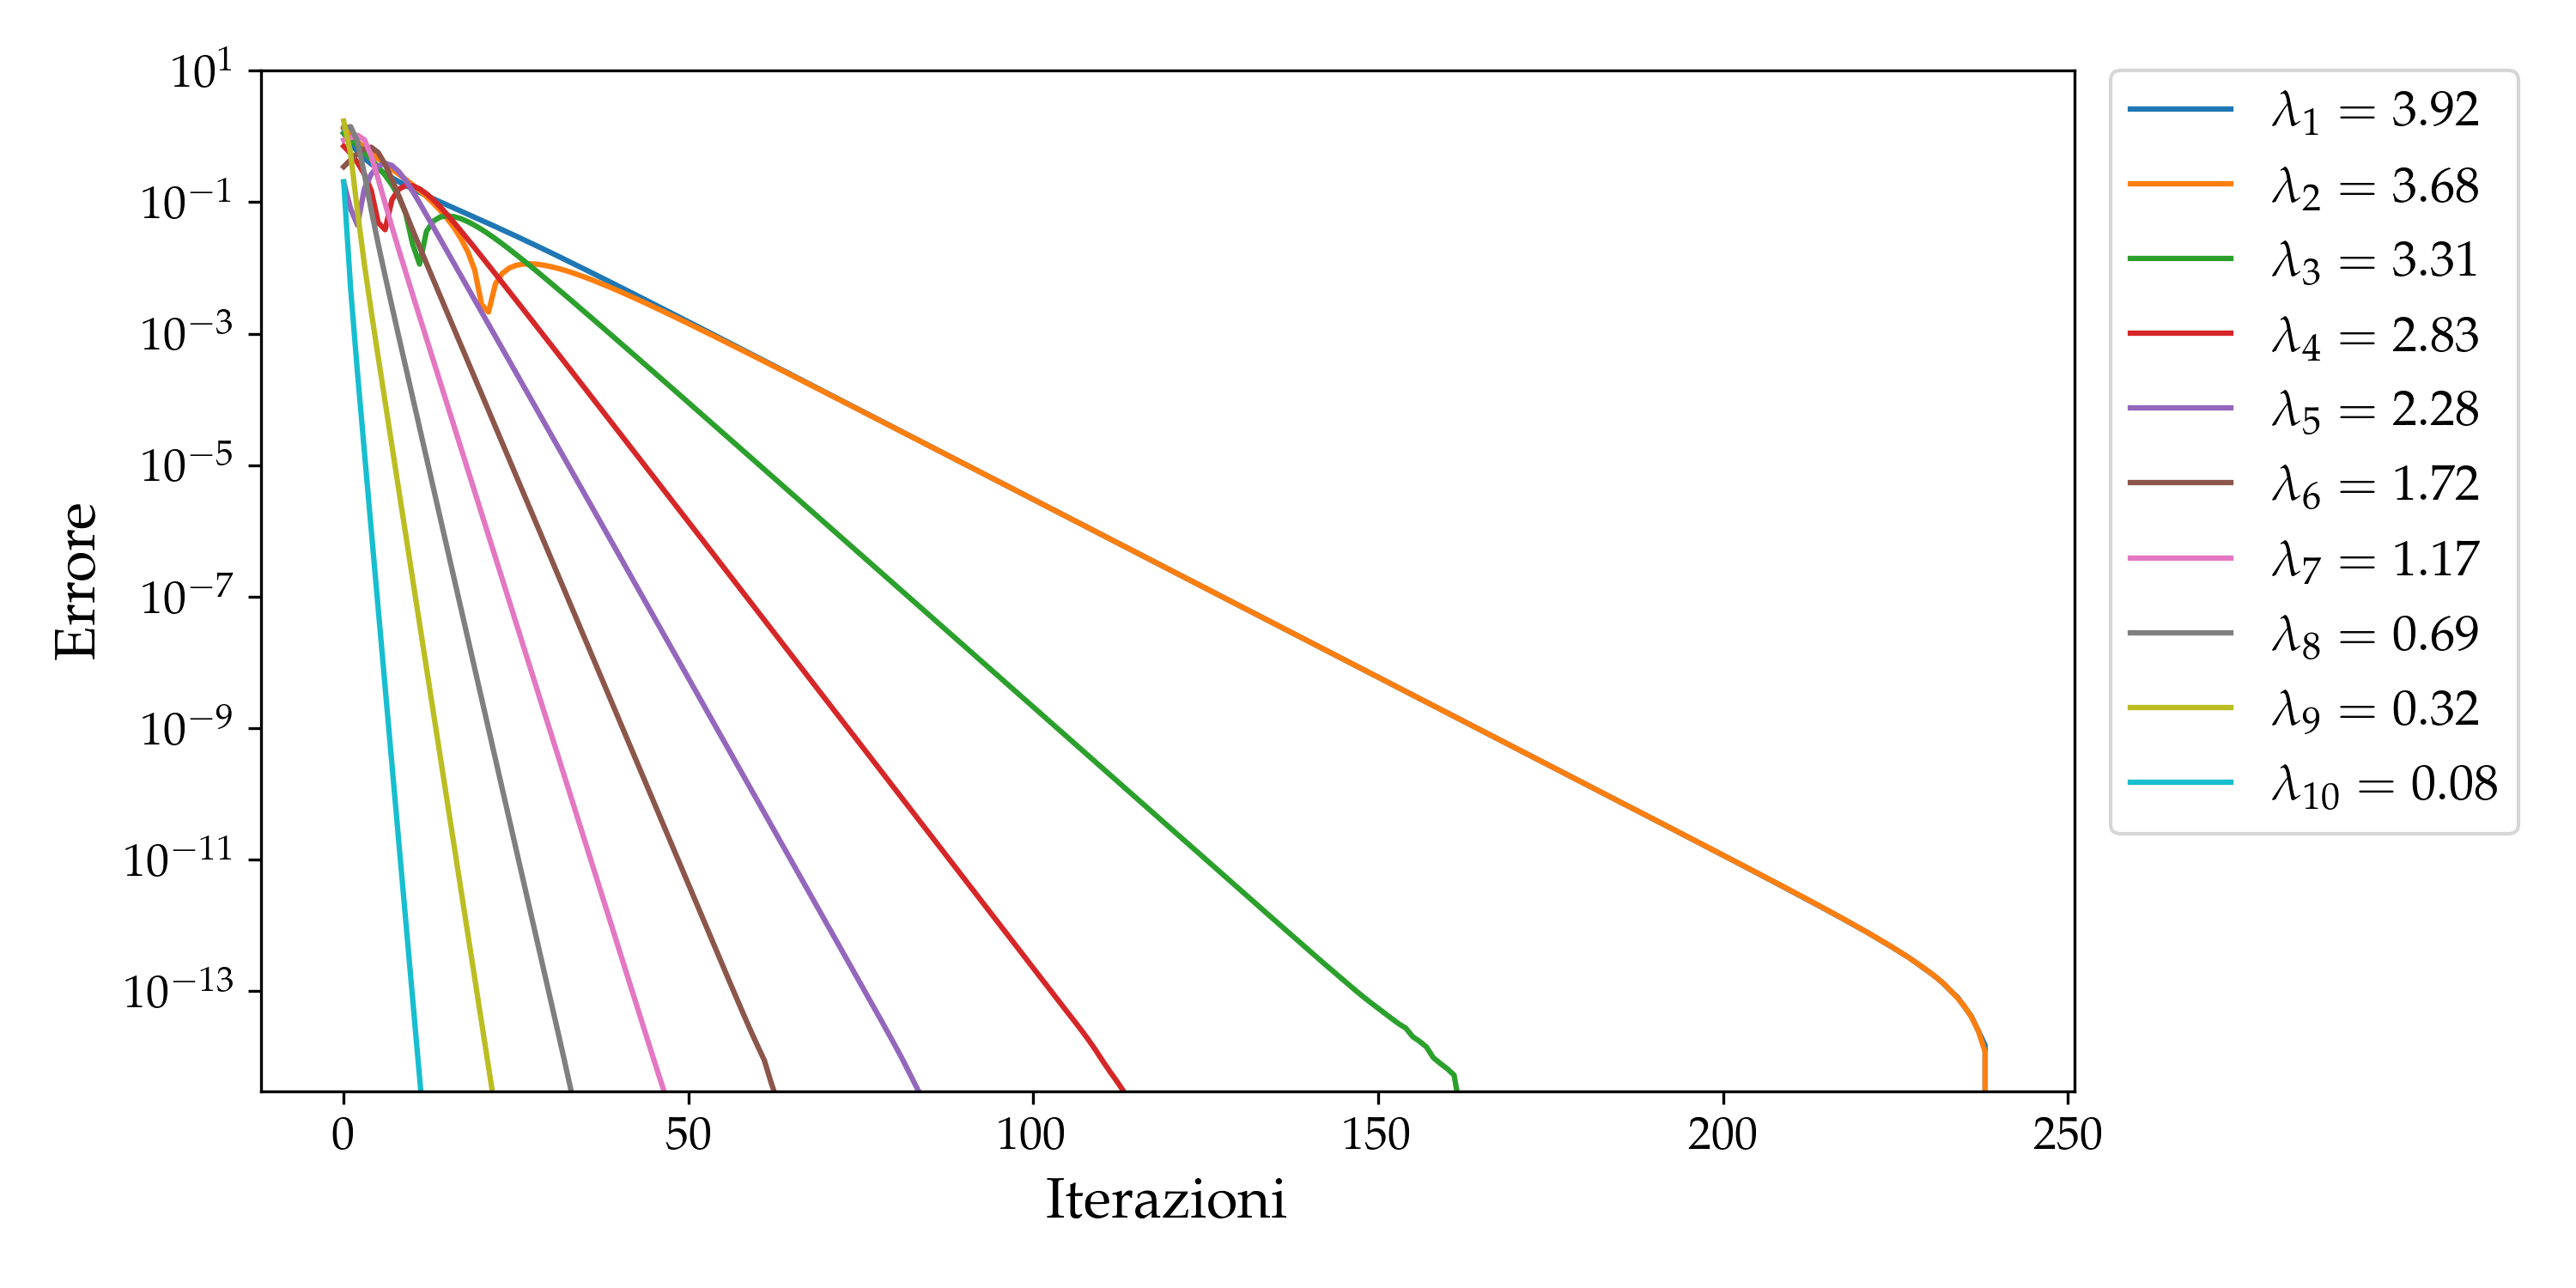
\includegraphics[width=0.7\linewidth]{images/7/conv_single_eigen.png}
    \caption{Andamento della convergenza per diversi autovalori di $K$.}
    \label{fig: Conv sing eigen}
\end{figure}




\newpage
\cleardoublepage 
\addtocontents{toc}{\bigskip\protect\textbf{\Large Interpolazione e Fitting}\par\smallskip}
\addtocontents{toc}{\protect\setcounter{tocdepth}{-2}} 
\part{\Huge Interpolazione e Fitting}
\addtocontents{toc}{\protect\setcounter{tocdepth}{2}} 
\section{Esercizio 4.1.1}

\subsection{Problem Statement}
Scrivi un programma che esegua la \textbf{Lagrange interpolation}. In questo caso, poiché i pesi sono precomputati, è particolarmente utile costruire una classe che li memorizzi internamente.

\begin{elegantcode}[title=Schema della classe Lagrange]
class Lagrange:
    property weights = calcolati quando la class viene inizializzata
    
    method eval = restituisce la interpolation alla posizione x
\end{elegantcode}

Testa la funzione sui seguenti set di dati:
\begin{enumerate}
    \item Dataset A
    \begin{elegantcode}
xA = np.array([0, 2, 3, 5, 7, 8, 10])
fA = np.array([0, 2, 2.5, 4, 2.5, 2, 0])
    \end{elegantcode}
    
    \item Dataset B
    \begin{elegantcode}
xB = np.array([0, 2, 3, 4, 5, 6, 7, 8, 10])
fB = np.array([0, 2, 2.5, 2, 4, 2, 2.5, 2, 0])
    \end{elegantcode}
    
    \item Dataset C
    \begin{elegantcode}
xC = np.array([0, 1, 2, 3, 4, 5, 6, 7, 8, 9, 10])
fC = np.array([0, 1.5, 2, 2.5, 2, 4, 2, 2.5, 2, 1.5, 0])
    \end{elegantcode}
\end{enumerate}

\subsection{Premessa Teorica}
Il problema che ci siamo posti è quello di trovare una curva che passi esattamente per dei punti fissati dalla richiesta, ricostruire quindi una forma analitica che ammetta per la controimmagine $\boldsymbol{x}$, immagine $\boldsymbol f$. Possiamo scegliere diversi tipi di interpolazioni, ci concentriamo su quelle lineari, cioè ricerchiamo:
\[
P(x) = \sum a_k\ \phi_k(x)\ , \quad P(x_i) = f_i\
\]

\noindent In particolare per una interpolazione Polinomiale:
\[
\phi_k(x) = x^k
\]

\subsection{Metodi Numerici e Algoritmi}

\subsubsection{Direct Method} \label{Cap: Direct Mth}
Il primo tentativo di interpolare dei punti con una curva può essere fatto implementando il cosiddetto \textit{Direct Method}: dato un set di $n$ punti $(x_i, f_i)$ si può introdurre una matrice $n\times n$ $V$ tale che
\[
f=aV
\]

\noindent scegliendo la base dei monomi $V$ è detta \textit{Matrice di Vandermonde}, così definita:
\[
V = \begin{pmatrix}
1 & x_1 & x_1^2 & \dots \\
1 & x_2 & x_2^2 & \dots \\
\dots
\end{pmatrix}
\]
A questo punto la ricerca del vettore dei coefficienti diventa la semplice risoluzione di un sistema lineare con la martice $V$, risolvibile agilmente con uno dei metodi che abbiamo precedentemente mostrato (Parte \ref{Cap: Matrici e Sistemi Lineari}).\\ 
\noindent Questa non risulta essere una buona soluzione alla ricerca del polinomio interpolante il sistema di punti generico, poiché si può dimostrare che al crescere del sistema la matrice diventa sempre più mal-condizionata. Un plot di seguito (Fig. \ref{fig: Vandermonde cond}) mostra il \textit{Condition Number} di $V$ in funzione del numero di punti da interpolare, che dimostra ciò a cui abbiamo appena fatto riferimento. 

\begin{figure}[H]
    \centering
    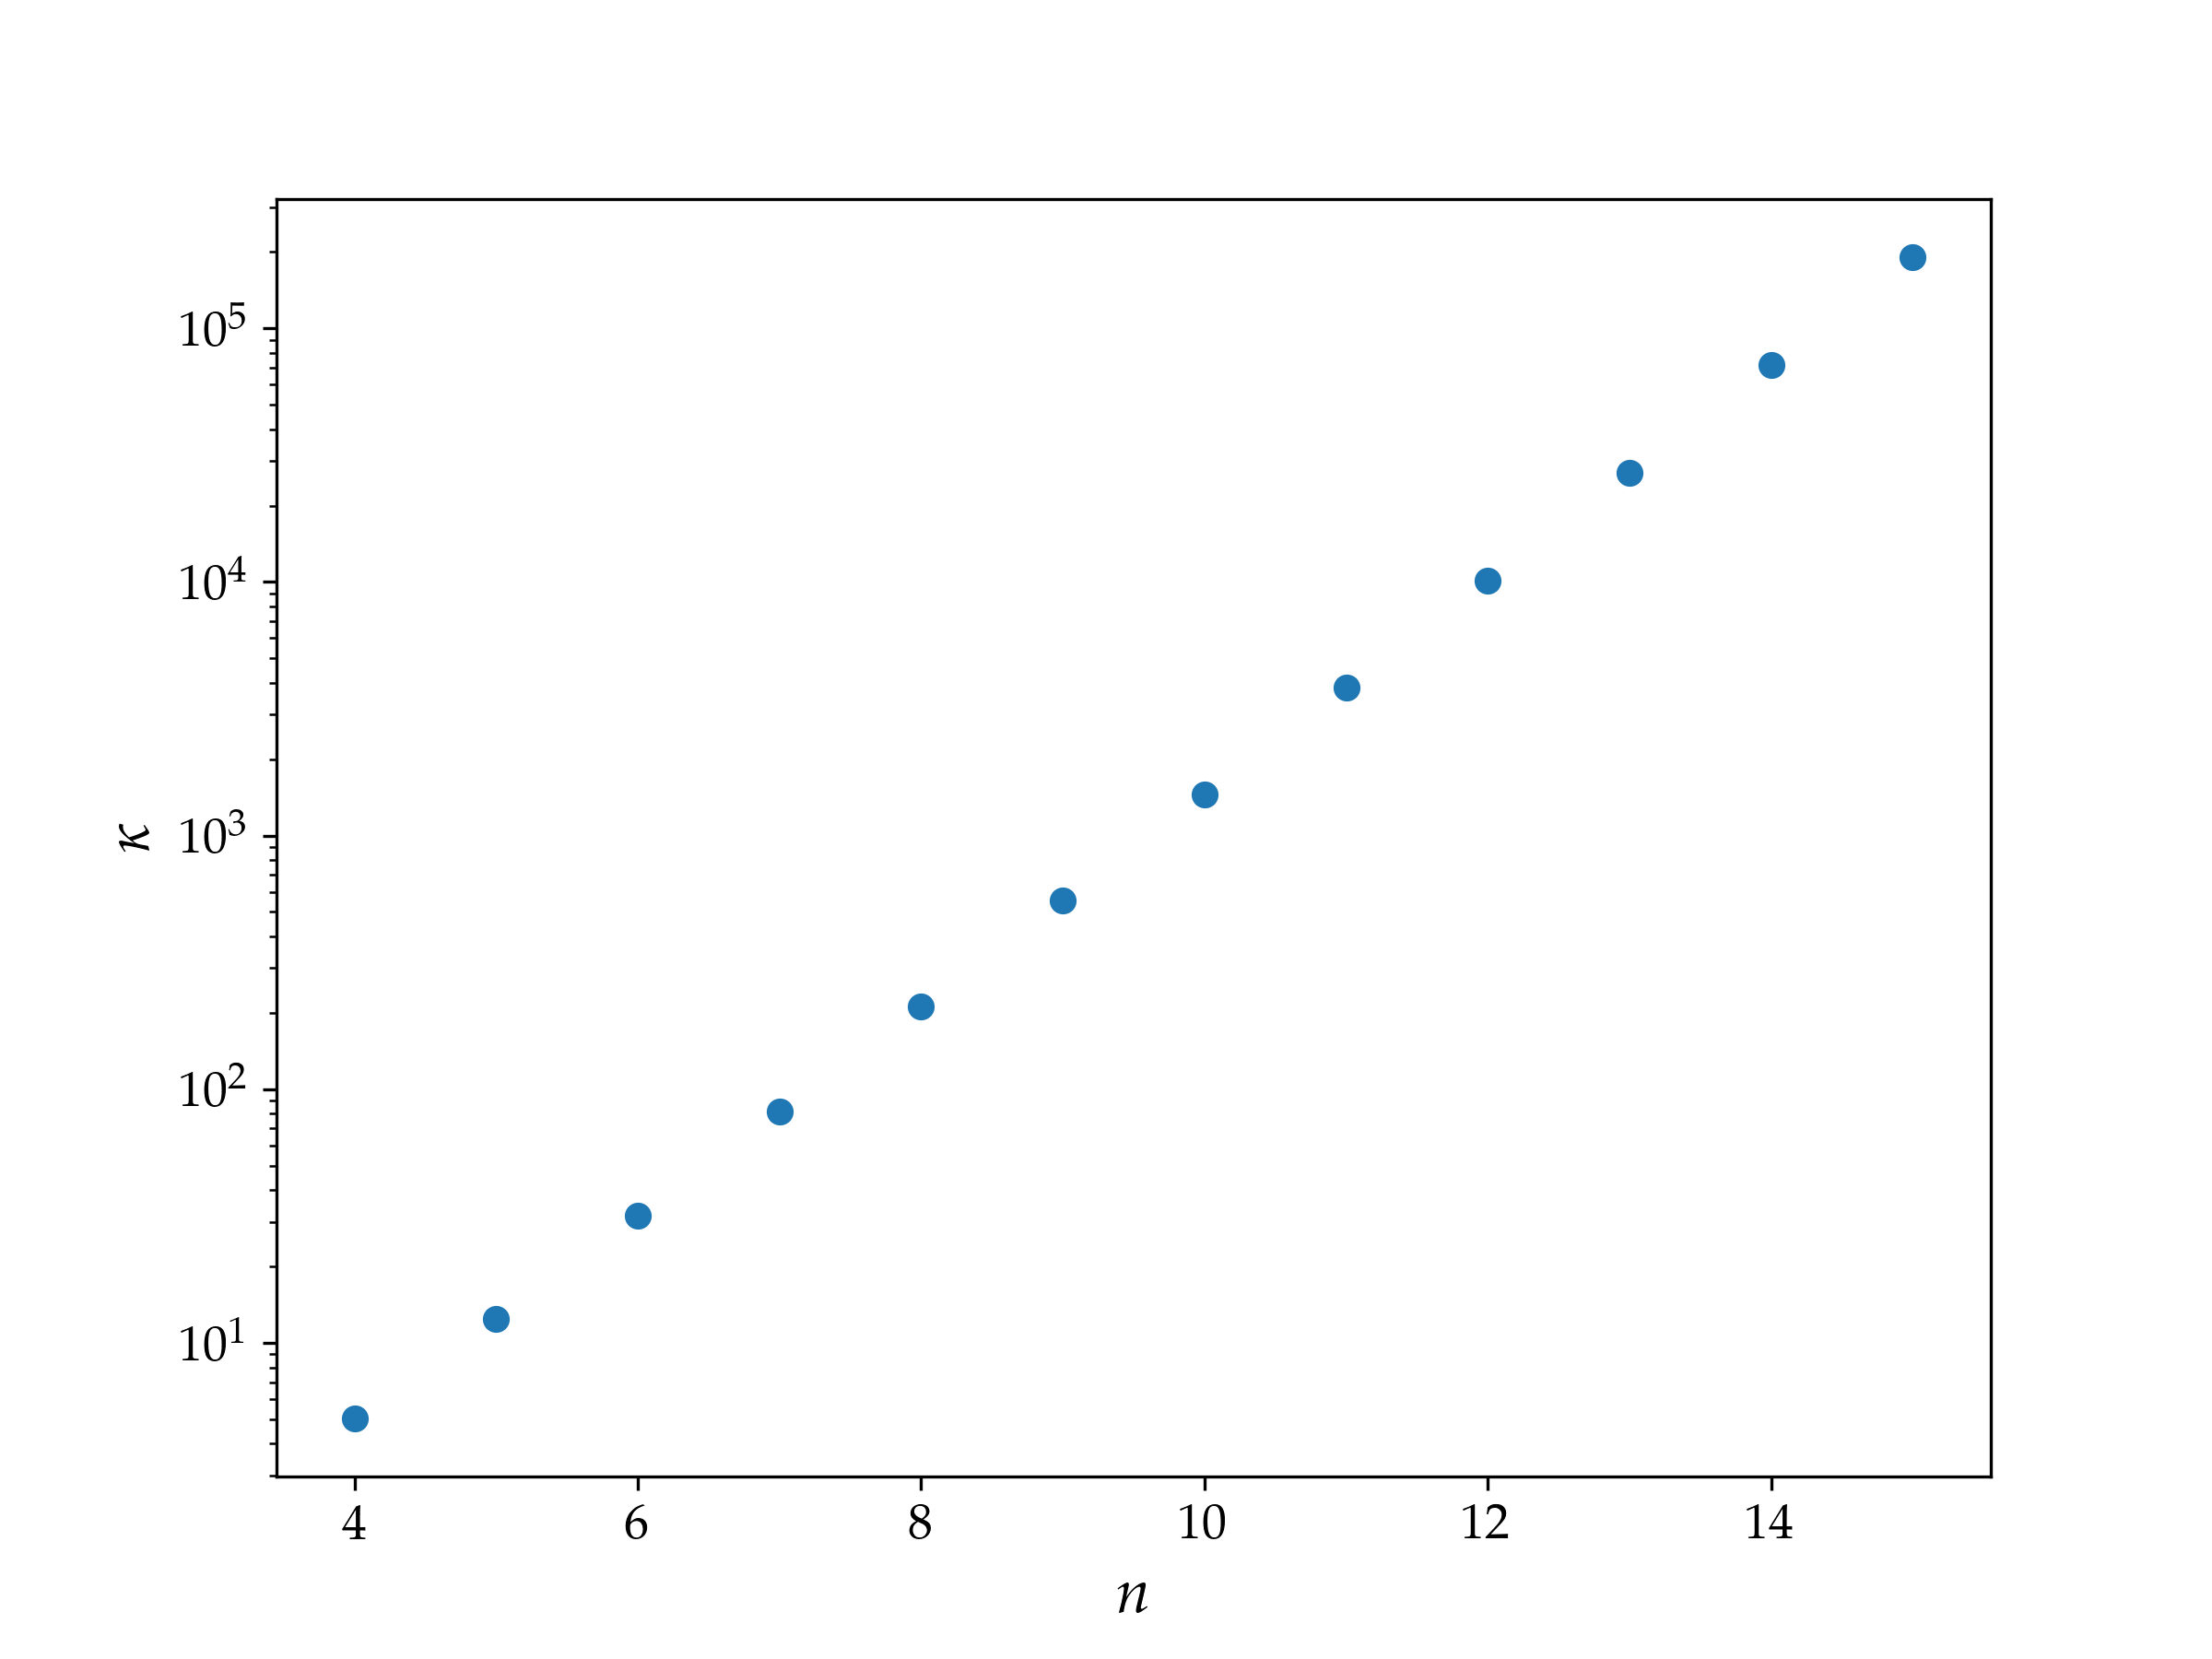
\includegraphics[width=0.7\linewidth]{images/8/Vandermonde_cond.png}
    \caption{\textit{Condition number} $\kappa$ della matrice di Vandermonde in funzione del numero di punti da interpolare $n$.}
    \label{fig: Vandermonde cond}
\end{figure}

\subsubsection{Lagrange Interpolation}
Un'alternativa è proposta dall'interpolazione di Lagrange, dove definiamo i \textit{Polinomi di Lagrange} $L_k(x)$:
\[
L_k(x) = \frac{\prod_{j=0, j \neq k}^{n-1}(x - x_j)}{\prod_{j=0, j \neq k}^{n-1}(x_k - x_j)} = w_k \prod_{j=0, j \neq k}^{n-1}(x - x_j)\
\]
\[
\frac{1}{w_k} = \prod_{j=0, j \neq k}^{n-1}(x_k - x_j) \quad \text{è una costante}
\]
La caratteristica principale di $L_k(x)$ è quella che 
\[
L_k(x_i) = \delta_{ki}
\]
quindi segue:
\[
P(x) = f = \sum a_k\ L_k(x) = \sum a_k \delta_{ki} = a_i
\]
Cioè la matrice di Vandermonde è l'identità, e non è necessario risolvere il sistema lineare poiché è banale. \\
Una riscrittura è possibile per ottimizzare il costo computazionale del problema:
\[
\begin{aligned}
P(x) = \dots = \left[ \sum_{k} \frac{f_k w_k}{(x - x_k)} \right] \left[ \sum_{k} \frac{w_k}{(x - x_k)} \right]^{-1}
\end{aligned}
\]

\noindent Si noti che nel calcolo del polinomio esattamente su un nodo si potrebbero incontrare problemi di divergenza del risultato numerico: risolviamo introducendo una piccola deviazione $\epsilon$, dell'ordine della \textit{machine precision}, trascurabile nel calcolo ordinario, ma che assicura alla nostra computazione, in questi casi più delicati, di non fallire

\[
\begin{aligned}
P(x) = \dots = \left[ \sum_{k} \frac{f_k w_k}{(x - x_k + \epsilon)} \right] \left[ \sum_{k} \frac{w_k}{(x - x_k + \epsilon)} \right]^{-1}
\end{aligned}
\]

\subsection{Risultati e Discussione}
L'uso di una classe risulta naturale, infatti il calcolo dei pesi è un'operazione da fare una sola volta, dato un certo set di punti, quindi essi possono essere computati e conservati.\\
Ho implementato questo tipo di logica nella mia soluzione:
\begin{elegantcode}
class Lagrange:
    def __init__(self, x, f):
        self.x = x
        self.f = f
        n = len(x)
        w_arr = []
        for k in range(n):
            mask = np.ones(len(x), dtype=bool)
            mask[k] = False
            wk = np.prod((x[k] - x[mask] + 1e-15))**(-1)
            w_arr.append(wk)
        self.w = np.array(w_arr)

    ...
\end{elegantcode}
\bigskip
\noindent Sono forniti 3 \textit{dataset}, vengono mostrati di seguito i punti nel piano (Fig \ref{fig: Repr dataset}) e la loro interpolazione con una curva, tramite metodo dei Polinomi di Lagrange (Fig \ref{fig: Lagrange interp}).

\begin{figure}[H]
    \centering
    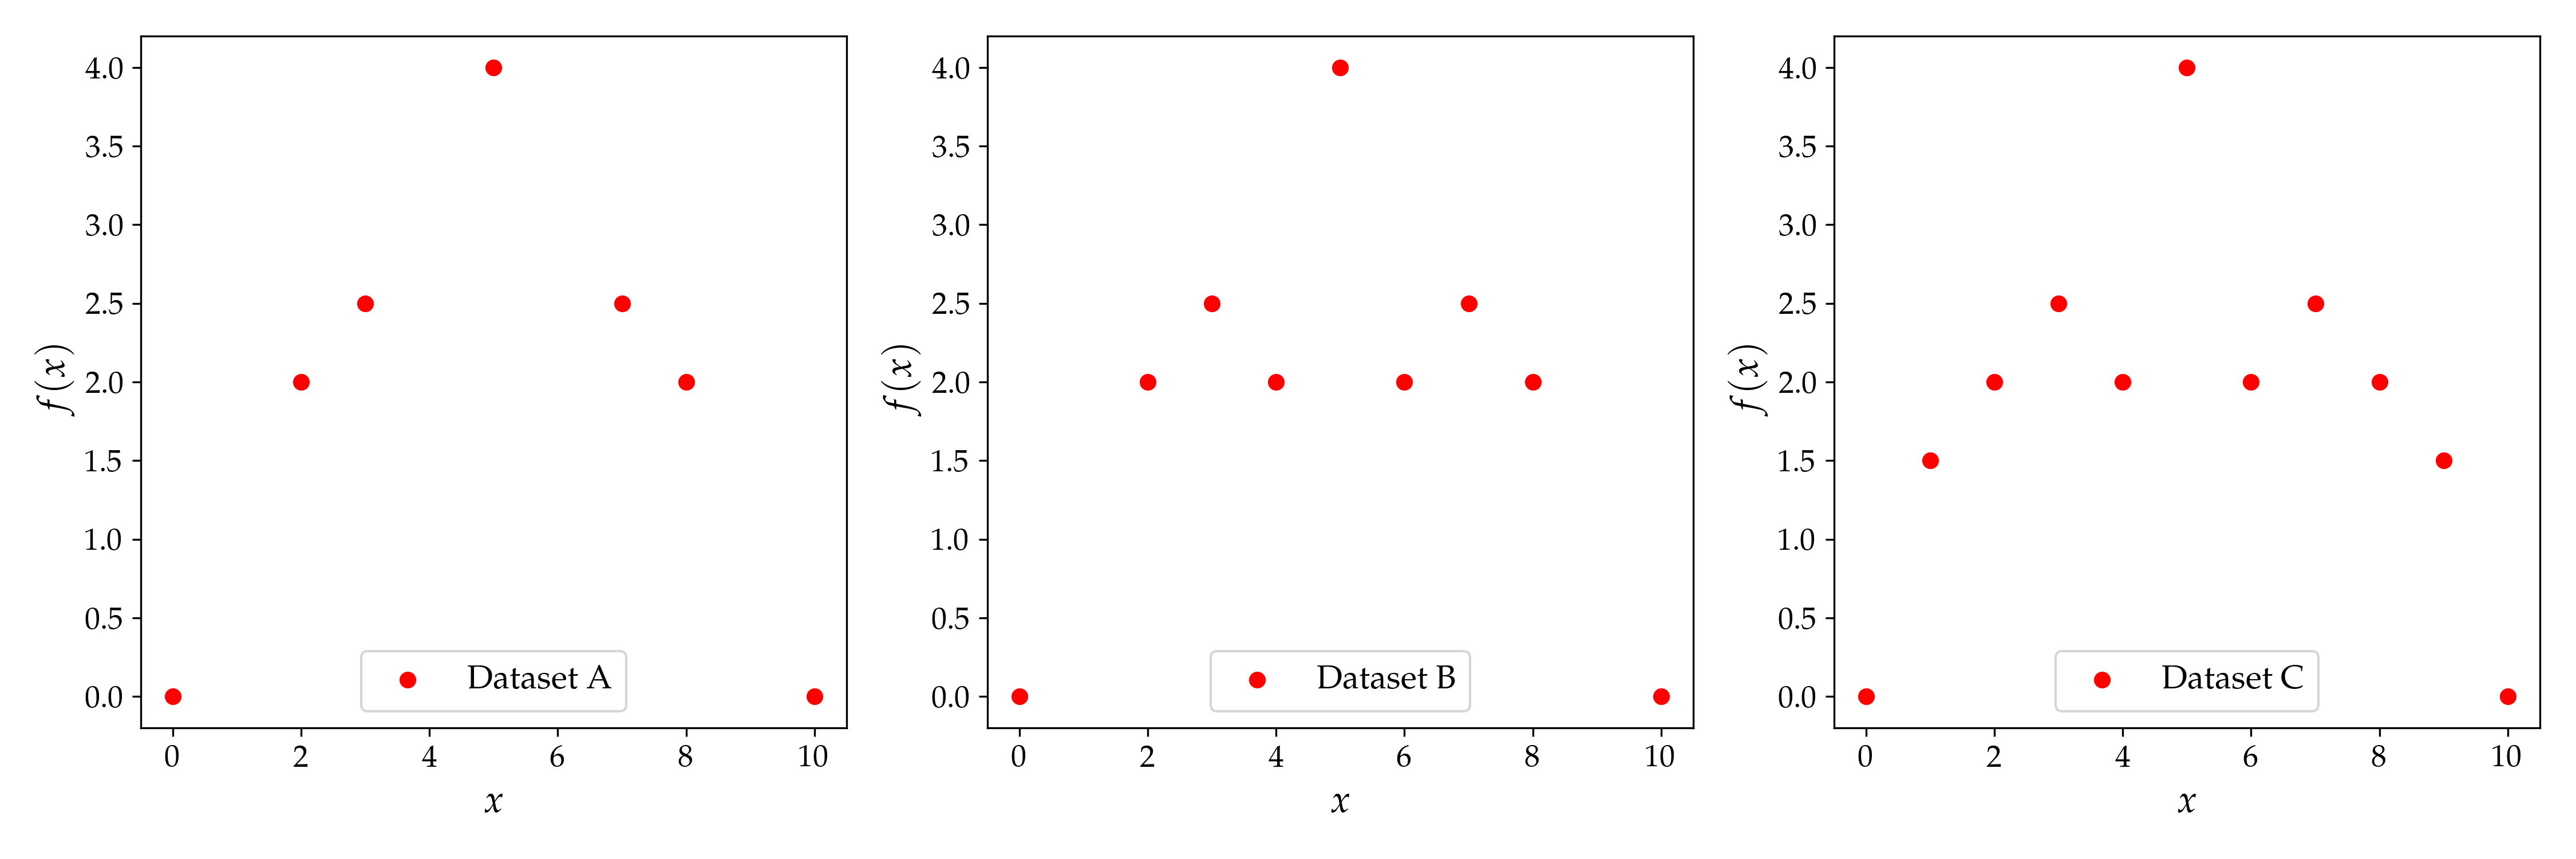
\includegraphics[width=\linewidth]{images/8/Lagrange_dataset_plot.png}
    \caption{Rappresentazione dei dataset.}
    \label{fig: Repr dataset}
\end{figure}

\begin{figure}[H]
    \centering
    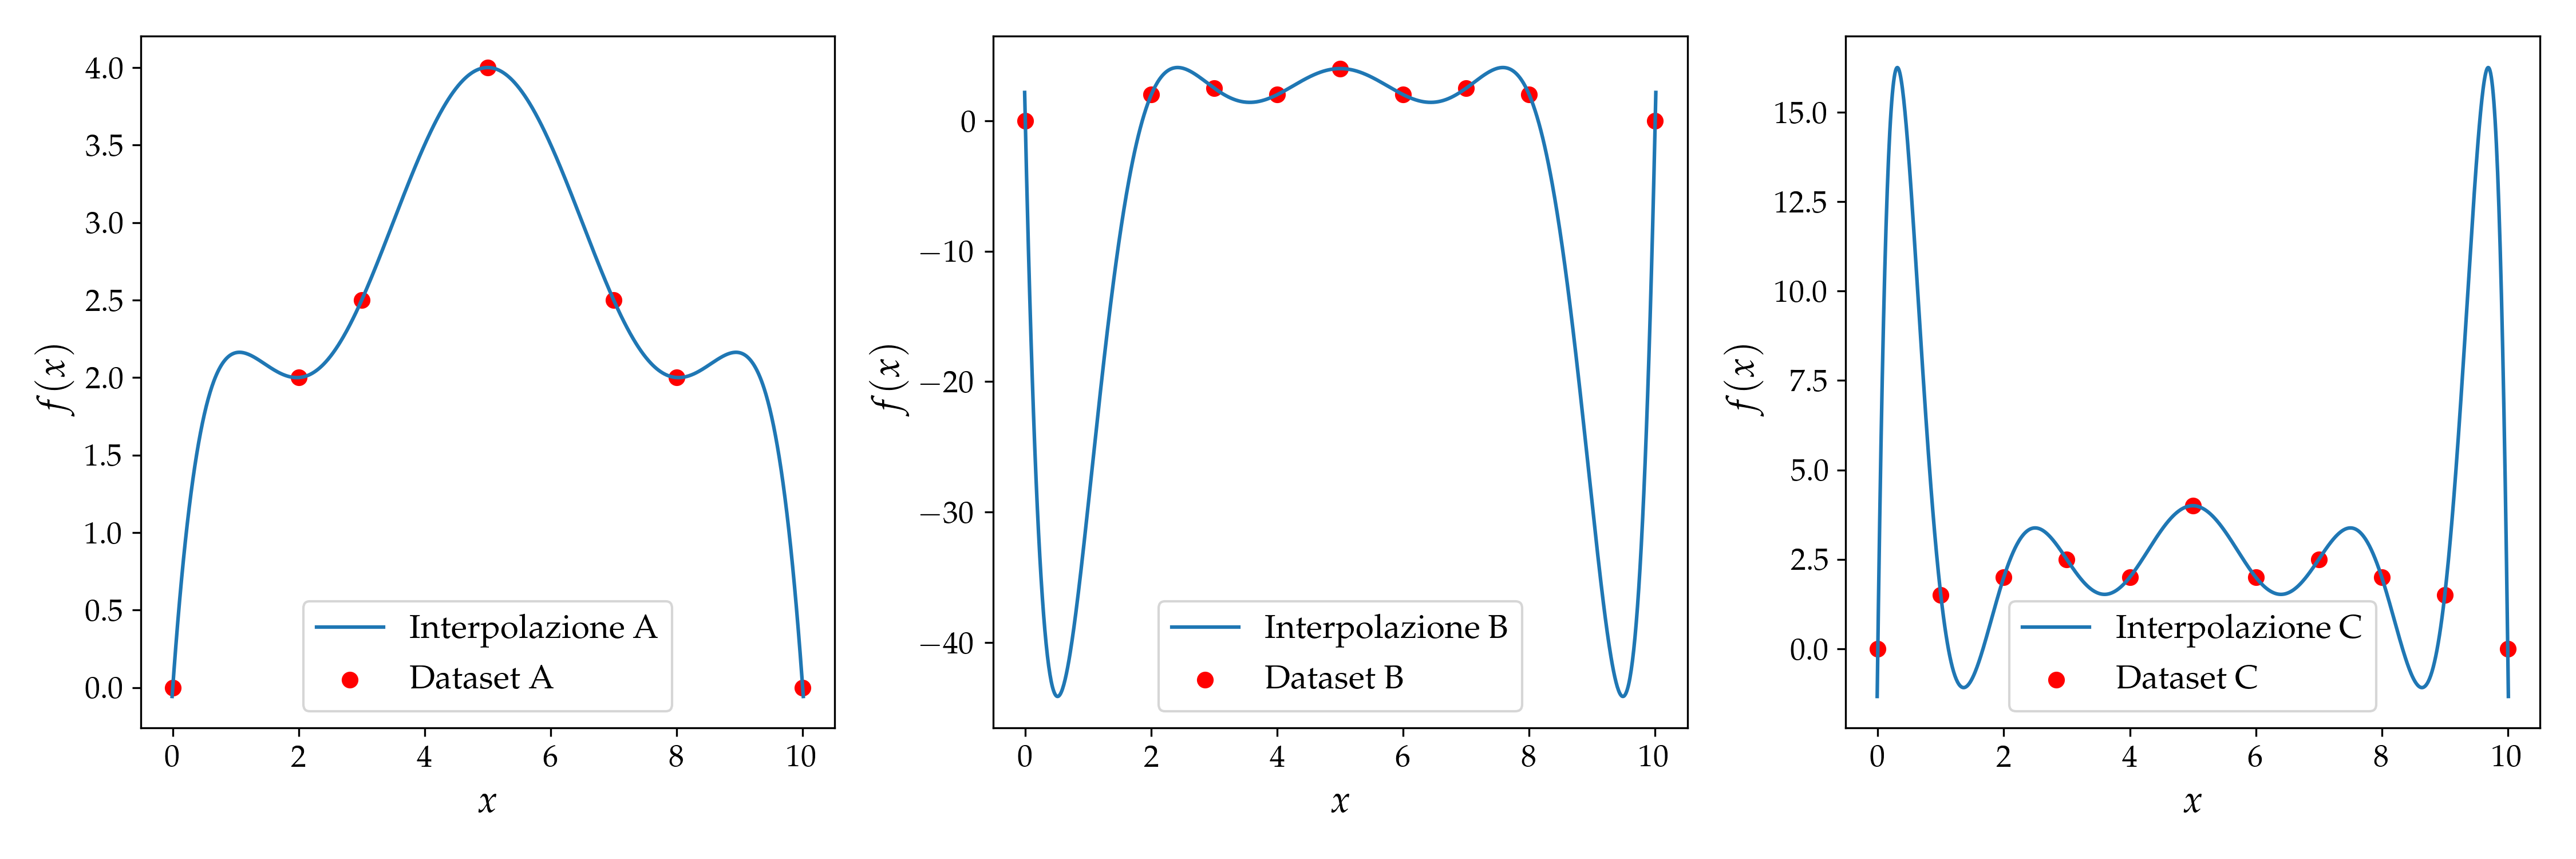
\includegraphics[width=\linewidth]{images/8/Lagrange_Interpolation.png}
    \caption{Interpolazione con \textit{Lagrange}.}
    \label{fig: Lagrange interp}
\end{figure}

\bigskip
\noindent Risulta interessante il confronto con l'interpolazione della curva tramite il \textit{Direct Method}. I problemi principali di questo approccio sono stati presentati nel Cap. \ref{Cap: Direct Mth}, ma qui vogliamo analizzare i risultati diretti di questa implementazione.

Nella Fig. \ref{fig: Dir mth interp} vediamo rappresentata la forma funzionale, polinomiale, trovata da questo secondo metodo e risulta evidente la similitudine con Fig. \ref{fig: Lagrange interp}.
\begin{figure}[H]
    \centering
    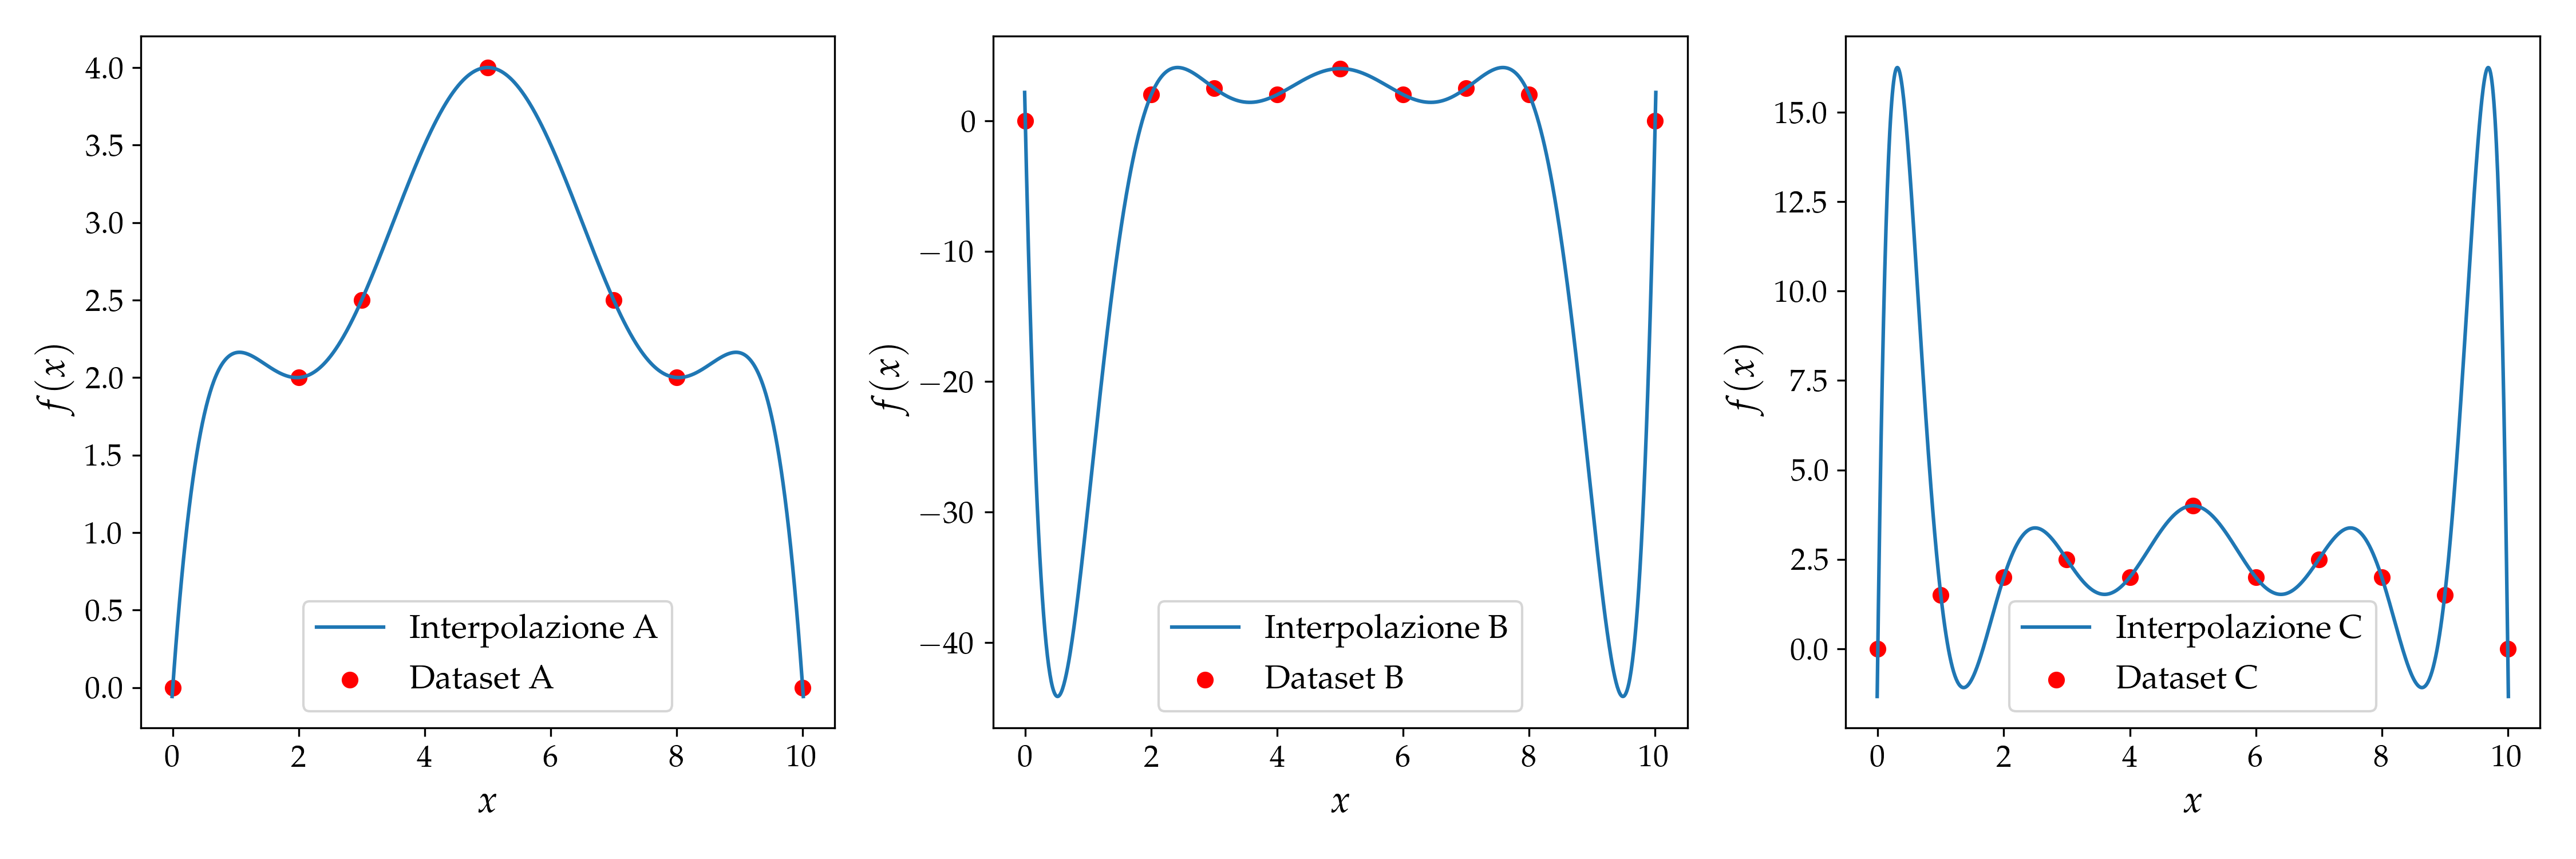
\includegraphics[width=\linewidth]{images/8/Direct_mth.png}
    \caption{Interpolazione con \textit{Direct Method}.}
    \label{fig: Dir mth interp}
\end{figure}

\noindent Una anlisi più precisa del fenomeno è possibile osservando l'errore assoluto tra le due descrizioni, definito come $|f_L(x) - f_D(x)|= E(x)$. Con riferimento al plot in Fig. \ref{fig: Err dir vs lag}, possiamo descrivere due andamenti differenti: se in prima analisi si osserva empiricamente una correlazione qualitativa tra l’andamento dell’errore e quello della funzione (ma senza una relazione generale), esiste un secondo \textit{slope} più interessante e preponderante nella parte destra del grafico. 

\medskip
\noindent Si osserva che $E(x)$ passa da un andamento regolare e ben definito a uno caratterizzato da oscillazioni sempre più pronunciate. Inoltre, l’ordine di grandezza dell’errore aumenta all’aumentare del numero di punti, mostrando una crescita approssimativamente esponenziale.

La spiegazione per queste osservazioni viene trovata nel mal condizionamento della \textit{Matrice di Vandermonde} e nel \textit{Direct Method}. Abbiamo mostrato già nel Cap.\ref{Cap: Direct Mth} come al crescesere del numero di punti, aumenti $\kappa$ per $V$, e questo spiega i diversi ordini di grandezza visibili sulla scala degli errori per i differenti dataset. 

Per quanto riguarda le oscillazioni della funzione, è necessario ricondursi alla definizione della matrice $V$, che contiene, nelle ultime colonne, termini dell'ordine di $x_i^N$, con $N$ numero di punti. Per N grande vengono molto amplificati gli errori sui coefficienti (instabilità numerica), inoltre le combinazioni di potenze con coefficienti di segno opposto porteranno a somme algebriche di numeri con diversi ordini di grandezza di differenza: questo lascia la possibilità per errori di arrotondamento legati alla \textit{machine precision}.

\medskip
\noindent Infine si può notare come spesso i minimi dell'errore si trovino in corrispondenza dei nodi, cioè dei punti in cui fissiamo il valore della funzione in maniera più rigida: le due interpolazioni saranno tendenzialmente più concordi sui valori qui assegnati.

\begin{figure}[H]
    \centering
    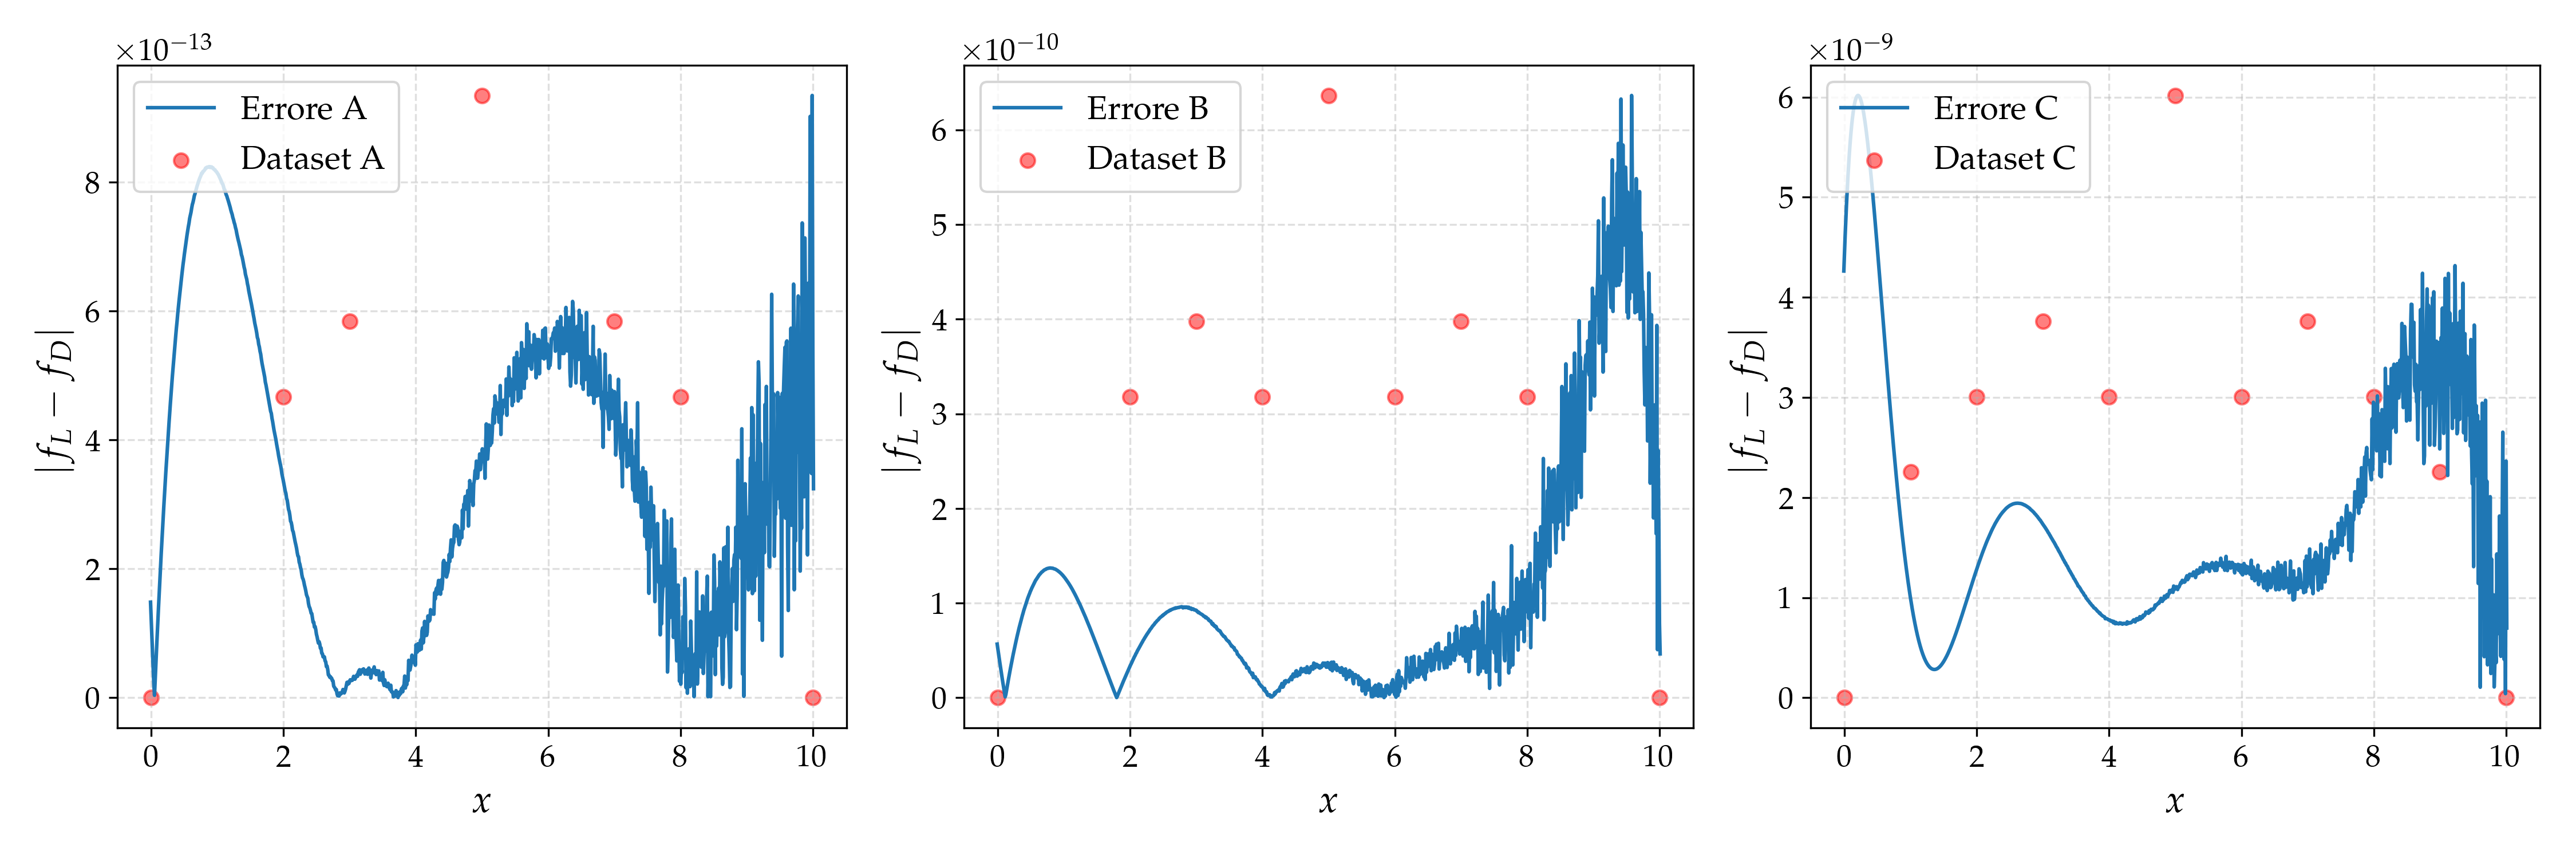
\includegraphics[width=\linewidth]{images/8/Err_dir_vs_lag.png}
    \caption{Plot dell'errore assoluto tra i metodi di \textit{Lagrange Interpolation} e \textit{Direct Method}, sui differenti dataset definiti in Fig. \ref{fig: Repr dataset}, che sono rappresentati in sovraimpressione, normalizzati per essere confrontabili con le dimensioni dell'errore.}
    \label{fig: Err dir vs lag}
\end{figure}
\newpage





\section{Esercizio 4.2.1}
\subsection{Problem Statement}
Si consideri la funzione di Runge
\[
\frac{1}{1 + 25x^2}.
\]
nel’intervallo $I=[-1,1]$. Calcolare la funzione interpolante utilizzando $N = 10, 20, 30, 40, 50$ nodi definiti sia come nodi equispaziati sia come nodi di Chebyshev. Utilizzare l’interpolatore basato sui polinomi di Lagrange e la \textit{monomial basis} (\textit{direct method} tramite matrice di Vandermonde).

\subsection{Premessa Teorica}
Nel contesto dell'interpolazione polinomiale di punti risulta interessante valutare le conseguenze date dal \textit{\textbf{Teorema di Stone-Weierstrass}}, che ci portano ad affermare che:
\begin{quote}
    ``Per un'interpolazione polinomiale, aumentando il numero di punti, cioè il grado del polinomio, è possibile aumentare anche l'accuratezza.''
\end{quote}

\noindent Ciò però non ci dice quale sia il metodo migliore nè stabilisce che tutti gli algoritmi siano equivalenti; l'esempio della funzione di Runge ci permette di mostrare l'efficacia di un modello diverso da quello utilizzato fin'ora negli esempi che abbiamo presentato. Si può mostrare come la scelta del sampling non uniforme con i \textit{nodi di Chebyschev} rappresenta un esempio di metodo che permette di risolvere il fenomeno di Runge.
 
\subsection{Metodi Numerici e Algoritmi}

\medskip
\noindent La funzione di Runge è definita come:
\[
f(x) = \frac{1}{1 + 25x^2}.
\]
ed è possibile mostrare come, per questo esempio, l'accuratezza della funzione interpolata, in $I$, diminuisca rispetto al modello al crescere del numero di punti che campioniamo, se scegliamo un campionamento uniforme. 

Un esempio in Fig. \ref{fig: Lag unif} dove il numero di nodi (uniformi) varia nell'intervallo $[10, 60]$ ed è possibile osservare come solo nell'intorno del massimo si migliori l'accuratezza; verso gli estremi accade il contrario, in maniera che la differenza con $f(x)$ sia assolutamente non trascurabile. 
Se definiamo i \textit{nodi di Chebyschev} come:
\[
x_j = -\cos \left( \frac{j\pi}{n-1} \right) \quad j = 0, 1 \dots n-1
\]
cioe come punti equidistanti su una circonferenza unitaria, ma proiettati sul suo diametro. Si può dimostrare che questo diventa un migliore sampling per l'intervallo $I$, come mostra il confronto con la Fig. \ref{fig: Lag Cheby}. I nodi di Chebyshev riducono l’errore massimo e, per funzioni regolari, favoriscono la convergenza dell’interpolante.

 \begin{figure}[H]
     \centering
     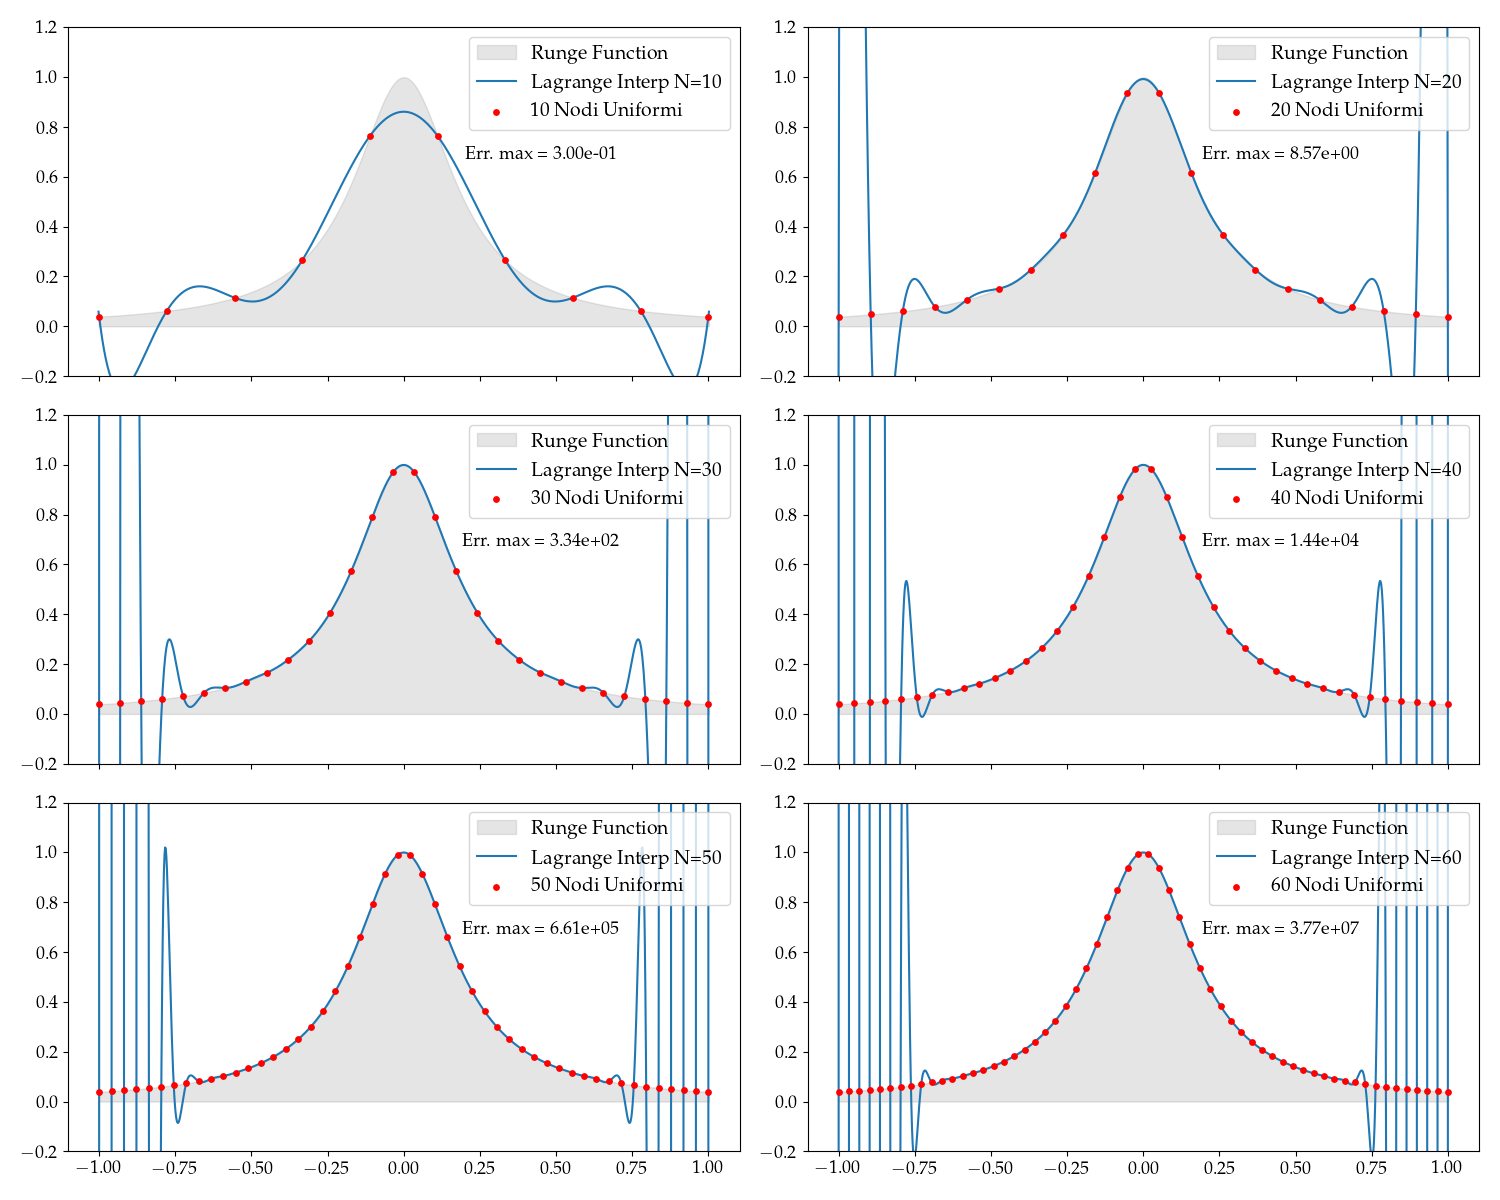
\includegraphics[width=\linewidth]{images/9/lagr_unif.png}
     \caption{\textit{Lagrange interpolation} di $f(x)$ in $[-1,1]$, nodi uniformi.}
     \label{fig: Lag unif}
 \end{figure}

\begin{figure}[H]
    \centering
    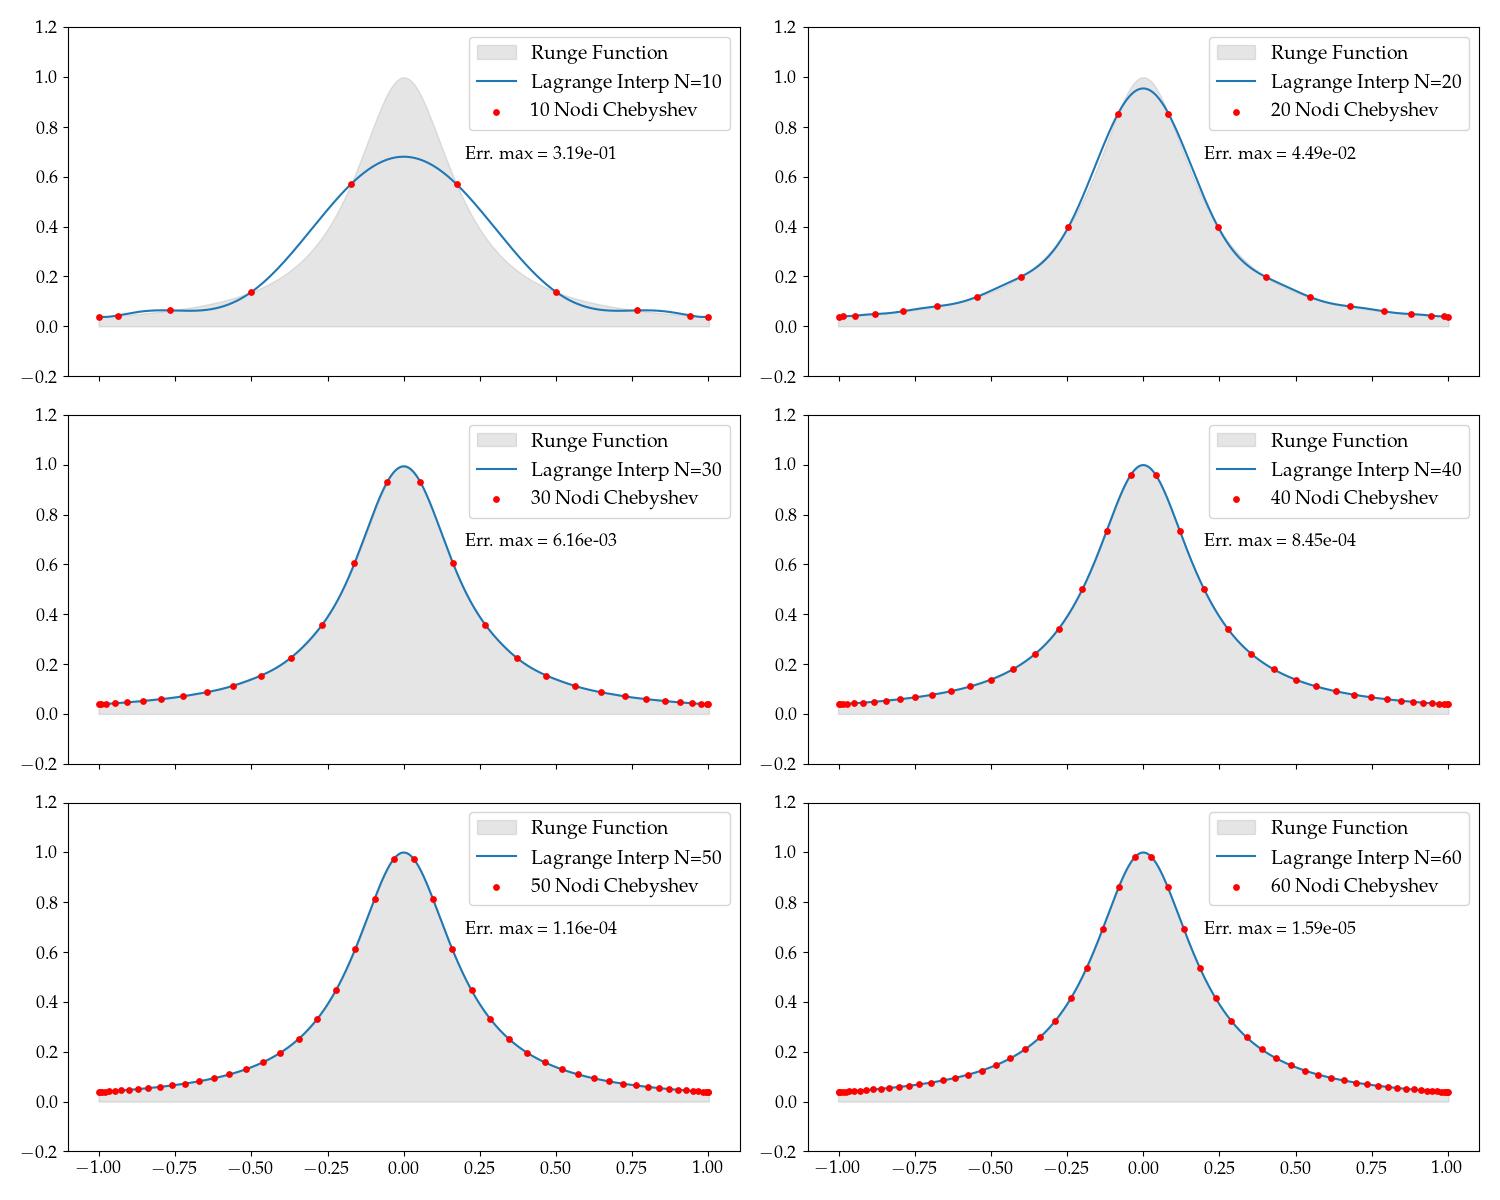
\includegraphics[width=\linewidth]{images/9/lagr_cheby.png}
    \caption{\textit{Lagrange interpolation} di $f(x)$ in $[-1,1]$, nodi di Chebyschev.}
    \label{fig: Lag Cheby}
\end{figure}
     
\subsection{Risultati e Discussione}
Le figure che abbiamo mostrato sottolineano la praticità e correttezza dell'utilizzo del sampling dei \textit{nodi di Chebyschev} per un algoritmo di intepolazione più accurato. \noindent Nelle stesse figure a cui avevamo fatto riferimento, indicato in sovraimpressione, abbiamo anche l'errore massimo nei nodi, nel confronto con $f(x)$: si osserva numericamente, nei plot di Fig. \ref{fig: Lag unif err} e Fig. \ref{fig: Lag cheby err} una crescita molto rapida (quasi esponenziale) che si ha all'aumentare del numero di nodi uniformi interpolanti, mentre un fenomeno opposto con i nodi di Chebyschev. 

\begin{figure}[H]
    \centering
    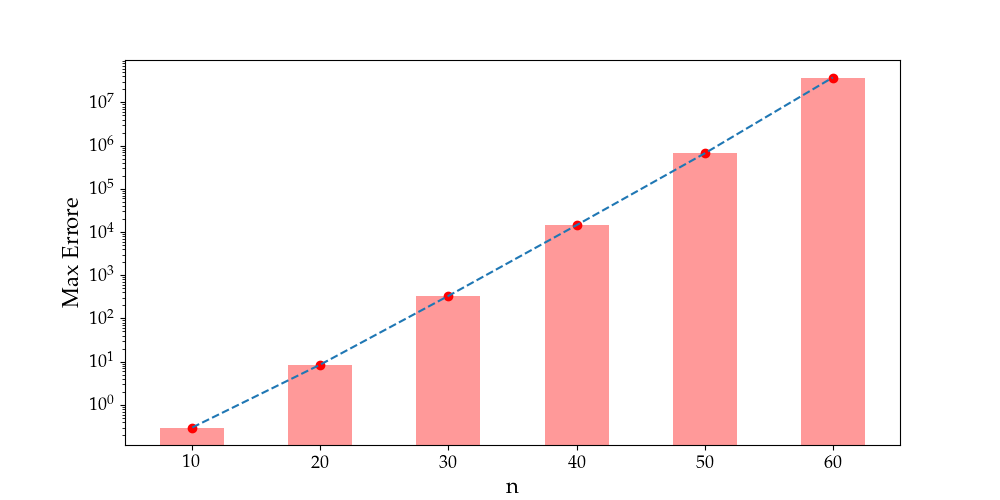
\includegraphics[width=0.8\linewidth]{images/9/unif_err.png}
    \caption{Errore massimo della funzione interpolata al variare del numero di nodi uniformi: è possibile osservare come l'\textit{Err Max} aumenti in maniera esponenziale, usando questo metodo.}
    \label{fig: Lag unif err}
\end{figure}

\begin{figure}[H]
    \centering
    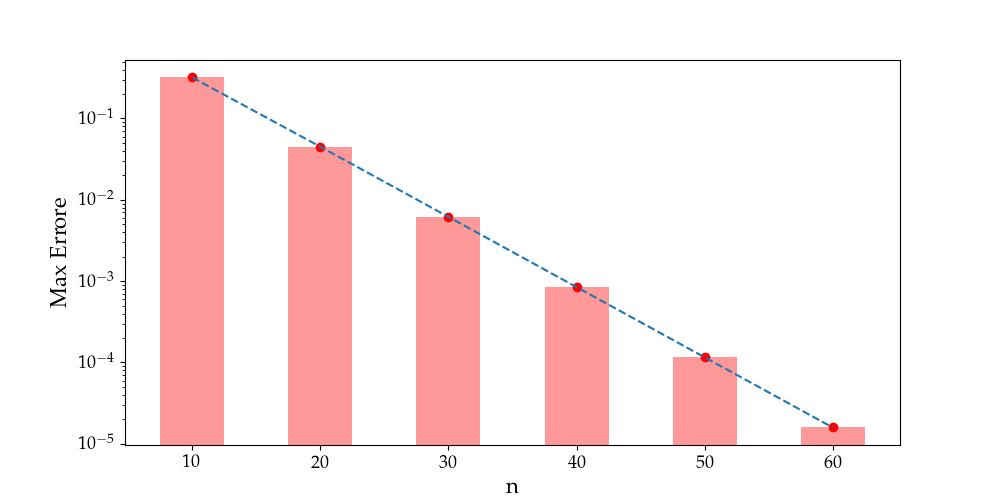
\includegraphics[width=0.8\linewidth]{images/9/cheby_err.png}
    \caption{Errore massimo della funzione interpolata al variare del numero di nodi di Chebyschev: vi è una decrescita esponenziale.}
    \label{fig: Lag cheby err}
\end{figure}

\noindent Infine ci interessa sottolineare che questo fenomeno non è proprio del metodo di interpolazione che abbiamo scelto, che per gli esempi precedenti era stato la \textit{Lagrange Interpolation}, difatti possiamo mostrare come anche per un metodo alternativo, scegliamo il \textit{Direct method}, è possibile mostrare lo stesso fenomeno di Runge.

\begin{figure}[H]
    \centering
    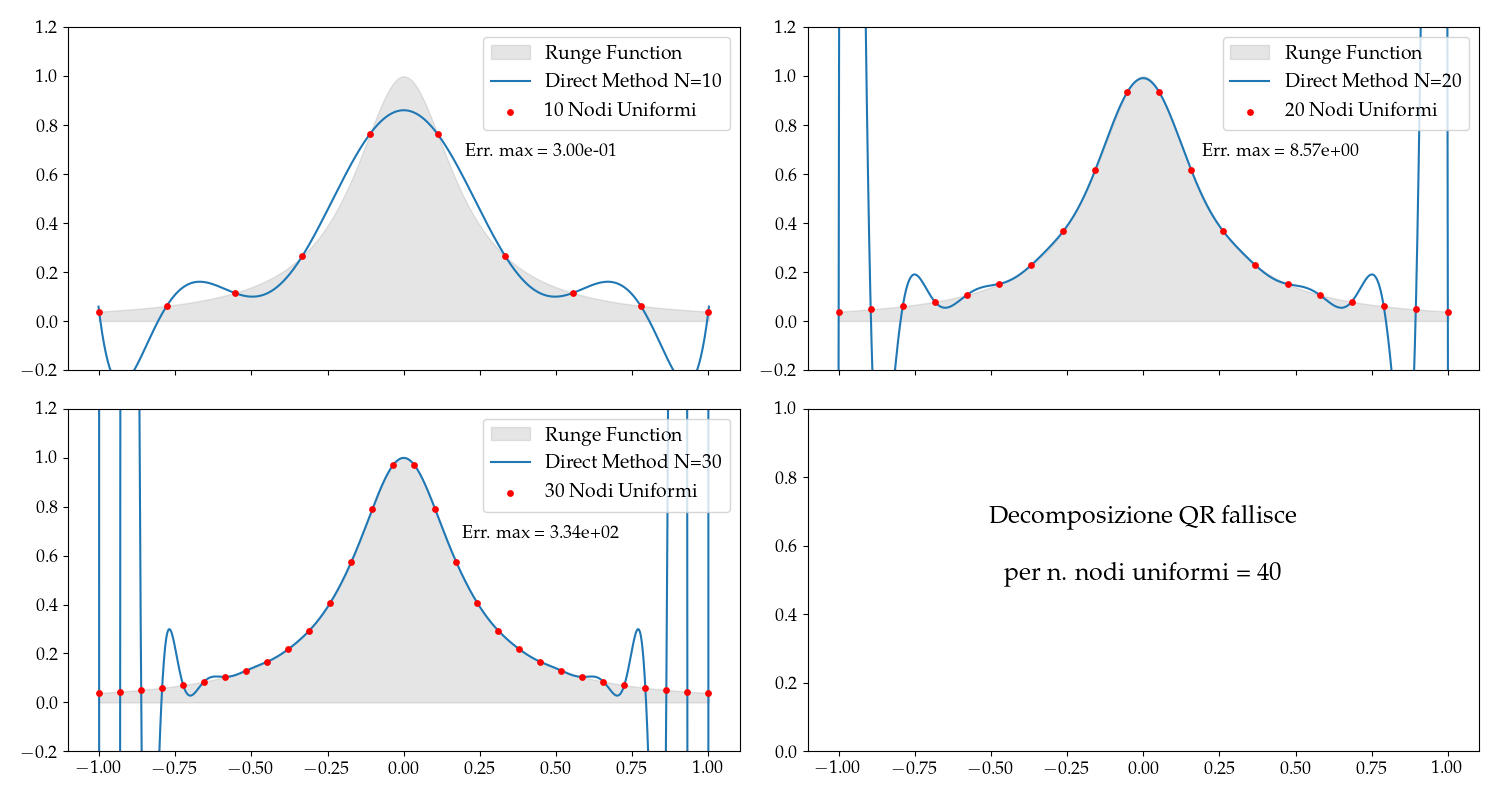
\includegraphics[width=0.8\linewidth]{images/9/direct_unif.png}
    \caption{\textit{Direct method} su $f(x)$ in $[-1,1]$, nodi uniformi. Sono note dal Cap. \ref{Cap: Direct Mth} le problematiche di questo metodo di interpolazione, che risultano più evidenti all'aumentare del numero di nodi: il risultato diventa numericamente instabile per $n \gtrsim 40$ a causa del mal condizionamento della matrice di Vandermonde.”}
    \label{fig: Direct unif}
\end{figure}

\begin{figure}[H]
    \centering
    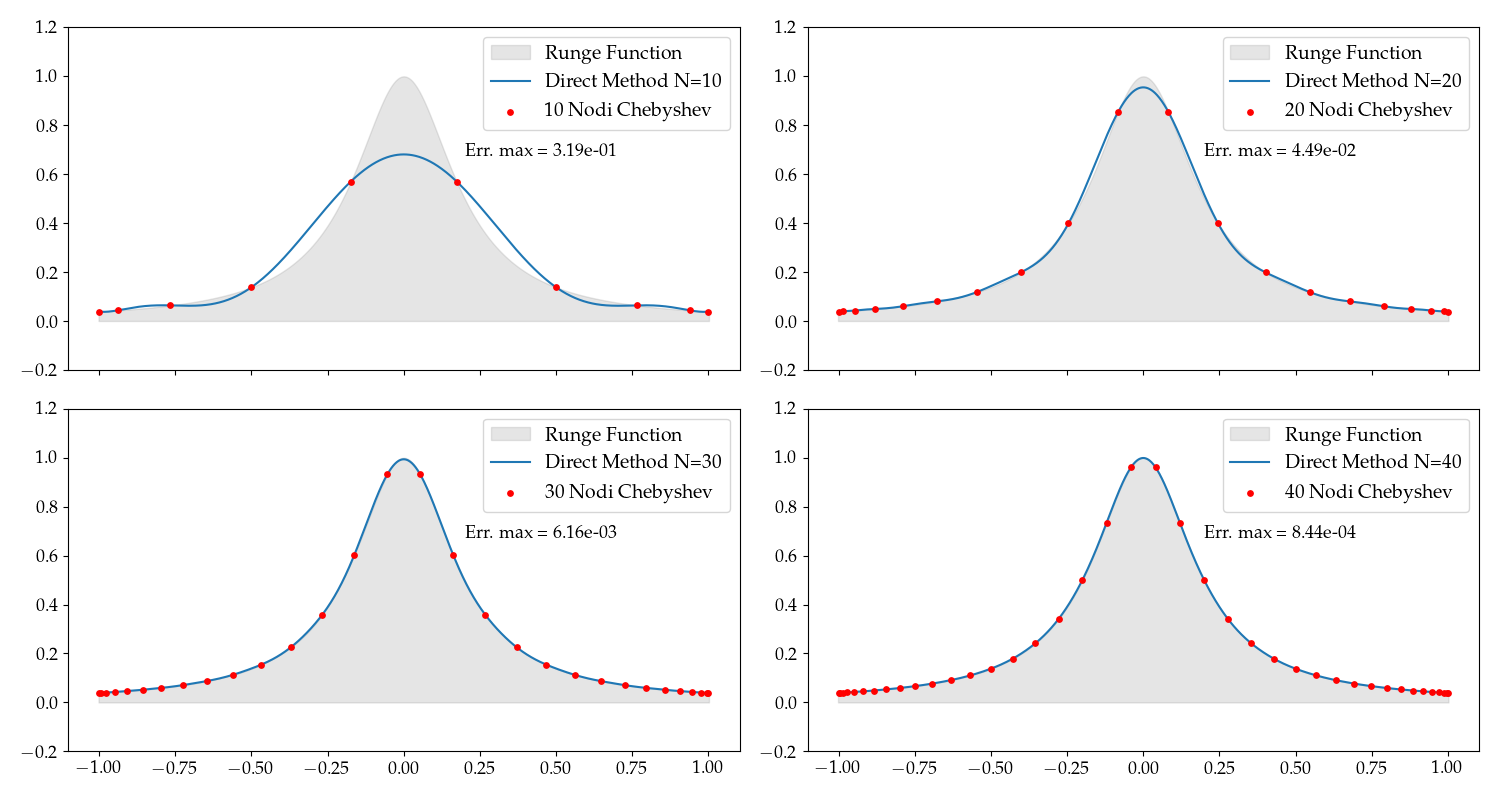
\includegraphics[width=0.8\linewidth]{images/9/direct_cheby.png}
    \caption{\textit{Direct method} su $f(x)$ in $[-1,1]$, nodi Chebyschev. Il metodo fallisce per $n \gtrsim 50$.}
    \label{fig: Direct cheby}
\end{figure}

\newpage








\section{Esercizio 4.4.1}
\subsection{Problem Statement}
Scrivi una classe che, dato l'insieme discreto di coordinate $x_i$, calcoli e memorizzi la matrice $W_{ij}$. 
Aggiungi i metodi \texttt{dft} e \texttt{idft}, entrambi i quali accettano un array della stessa lunghezza di $\{x_i\}$ 
e restituiscono la DFT diretta o inversa (internamente i due metodi applicano 
la matrice $W$ o la sua aggiunta $W^\dagger$). Partendo dai seguenti parametri:
\begin{itemize}
    \item $L = 2\pi$
    \item $N = 128$
    \item $\alpha = 0.5$
    \item $u(x, 0) = \sin(x) + 0.5 \sin(3x)$
\end{itemize}

\noindent Risolvi l'equazione del calore 1D implementando questi passaggi:
\begin{enumerate}
    \item Applica la DFT diretta a $u(x, 0)$ e calcola $\tilde{u}(k, 0)$
    \item Calcola $\tilde{u}(k, t)$
    \item Applica la DFT inversa a $\tilde{u}(k, t)$ per trovare $u(x, t)$
\end{enumerate}

\noindent Ripeti questa operazione per 20 valori di $t \in [0, 2]$ e poi plottali insieme.

\subsection{Premessa Teorica}
\subsubsection{Interpolazione Trigonometrica}
nei capitoli precedenti ci siamo occupati di interpolazioni lineari, cioè in cui vale che:
\[
P(x) = \sum a_k \phi_k(x)
\]
in particolare scegliendo $\phi_k(x) = x^k$, cioè definendo un'interpolazione polinomiale. Un'alternativa a questo approccio è data da un'interpolazione trigonometrica, cioè in cui $\phi_k(x) = e^{ikx} = \omega^k, \quad \omega = e^{ix}$. Questa diventa un'estensione complessa della base dei monomi, permettendo di estendere anche il teorema di unicità, che affermava:

\bigskip
\noindent Dato l'insieme di $N$ punti $x_k = 2\pi k/N$, con $k = 0, 1 \dots N - 1$, per ogni insieme di punti di supporto $(x_k, f_k)$, con $f_k$ complesso, esiste un unico polinomio

\[
P(x) = \sum_{k=0}^{N-1} a_k e^{ikx}
\]

\noindent che soddisfa $P(x_k) = f_k$ per ogni $k$. Definendo $\omega_k = e^{ix_k} = e^{2\pi i k/N}$, i coefficienti possono essere calcolati esplicitamente utilizzando

\[
a_k = \frac{1}{N} \sum_{j=0}^{N-1} f_j \omega_j^{-k} = \frac{1}{N} \sum_{j=0}^{N-1} e^{-2\pi ijk/N} f_j
\]

\noindent In genere, i coefficienti $a_k$ sono chiamati la trasformata di Fourier di $f$ e vengono indicati con $\tilde{f}_k$.
Definendo $\Delta x = L/N$, cioè il passo di sampling regolare su un intervallo $[0, L]$, definiamo la \textit{Trasformata di Fourier diretta} (DFT):
\[
\tilde{f}(p) = \Delta x \sum_{i=0}^{N-1} f(x_i) e^{ipx_i}
\]
dove p è il momento, cioè la coordinata nello spazio di Fourier. La trasformata inversa (IDFT) diventa quindi:
\[
f(x_i) = \frac{1}{L} \sum_{j=0}^{N-1} e^{-ip_j x_i} \tilde{f}(p_j)
\]

\subsubsection{Equazione del calore 1D}
In particolare la FT ci viene in aiuto come metodo standard per risolvere alcuni tipi di equazioni differenziali: nello spazio dei momenti la derivata rispetto alle coordinate diventa un semplice prodotto, semplificando molto il calcolo, in particolare consideriamo l'equazione del calore 1D su un dominio $x \in [0, L]$ con condizioni al contorno periodiche:

\begin{equation} \label{eq: Heat eq}
\frac{\partial u}{\partial t} = \alpha \frac{\partial^2 u}{\partial x^2}, \quad u(x, 0) = f(x)
\end{equation}

\begin{itemize}
    \item $u(x, t)$ è la temperatura alla posizione $x$ e al tempo $t$,
    \item $\alpha$ è la diffusività termica,
    \item $f(x)$ è la distribuzione iniziale di temperatura.
\end{itemize}

se valutiamo la trasformata del lato sx e dx:
\begin{itemize}
    \item $\mathcal{F} \left[ \frac{\partial u}{\partial t} \right] = \frac{\partial \tilde{u}}{\partial t}$
    \item $\mathcal{F} \left[ \frac{\partial^2 u}{\partial x^2} \right] = -p^2 \tilde{u}$
\end{itemize}

quindi l'equazione si riduce ad una ODE:
\[
\frac{\partial \tilde{u}}{\partial t} = -\alpha p^2 \tilde{u}
\]

la cui soluzione analitica è:
\[
\tilde{u}(p,t) = \tilde{u}(p,0) e^{-\alpha p^2t}
\]
La condizione sul valore iniziale è nota, risulta sufficiente calcolare la trasformata del valore iniziale; abbiamo quindi la soluzione nello spazio dei momenti, basta una IFT per tornare nello spazio delle coordinate e risolvere Eq. \ref{eq: Heat eq}
\[
\tilde{u}(p,t) \longrightarrow u(x,t)
\]

\subsection{Metodi Numerici e Algoritmi}
Per implementare la risoluzione del problema proposto risulta naturale passare ad una espressione matriciale della definizione della DFT e IDFT:
\[
\tilde{f}_k = \Delta x \sum_{i} W_{ki} f_i \quad \quad W_{ki} = e^{i p_k x_i}
\]
Questo offre la possibilità di usare gli algoritmi già sviluppati per la risoluzione dei sistemi lineari, in più permette un semplice passaggio da DFT a IDFT, che necessiterebbe di invertire $W$, ma che diventa il banale calcolo di $W^\dagger$:
$$W^\dagger W = N I \implies W^{-1} = \frac{1}{N} W^\dagger \implies W^\dagger = N W^{-1}$$
quindi:
\[
\tilde{f}_k = \Delta x \sum_{i} W_{ki} f_i \quad \quad f_i = \frac{1}{L} \sum_{k} W^\dagger_{ik} \tilde{f}_k 
\]

\medskip
\noindent Questa la classe che abbiamo implementato nel nostro codice \textit{.py}:
\begin{elegantcode}
class DFT:
    def __init__(self, x_desc):
        N = len(x_desc)
        L = (x_desc[-1] - x_desc[0])
        
        if N % 2 == 0: 
            p_pos = np.arange(N//2+1)   # positive values bcs of Niquist (even)
            p_neg = np.arange(1, N - (N//2)) * (-1)
        else: 
            p_pos = np.arange(N//2)     # positive values bcs of Niquist (odd)
            p_neg = np.arange(1, N - (N//2)) * (-1)

        p = 2 * np.pi / L * np.concatenate((p_pos, p_neg))
        W = np.exp(1j * np.outer(p, x_desc))

        self.W = W
        self.p = p
        self.N = N
        self.L = L
        self.dx = L / N
    
    def dft(self, y_desc):
        if type(y_desc)==int or len(y_desc) != self.N:
            raise ValueError('len(y_desc) must be equal to len(x_desc)!')
        y_dft = self.dx * self.W @ y_desc
        return y_dft

    def idft(self, y_desc):
        if type(y_desc)==int or len(y_desc) != self.N:
            raise ValueError('len(y_desc) must be equal to len(x_desc)!')
        y_idft = self.L**(-1) * self.W.conj().T @ y_desc
        return y_idft
    
\end{elegantcode}

\subsection{Risultati e Discussione}
L'esercizio permette un'efficace rappresentazione grafica tramite la libreria \textit{matplotlib}, in particolare con l'uso di mappe di colore e curve di livello, che esprimono il variare della $u(x,t)$. Sono mostrate due rappresentazioni differenti del fenomeno: in Fig. \ref{fig: Heat 2d} è dato un plot in cui segnamo diverse curve di livello, corrispondenti ai 20 valori temporali per cui valutiamo la funzione, ogni curva ha assegnato un colore, proprio di un valore temporale. In Fig. \ref{fig: Heat 3d} la rappresentazione è 3d, dove lungo l'asse x e y troviamo $x$ e $t$, mentre l'asse z riporta il valore di $u(x,t)$, anche il colore riporta l'informazione sul valore di $u$.



\begin{figure}[H]
    \centering
    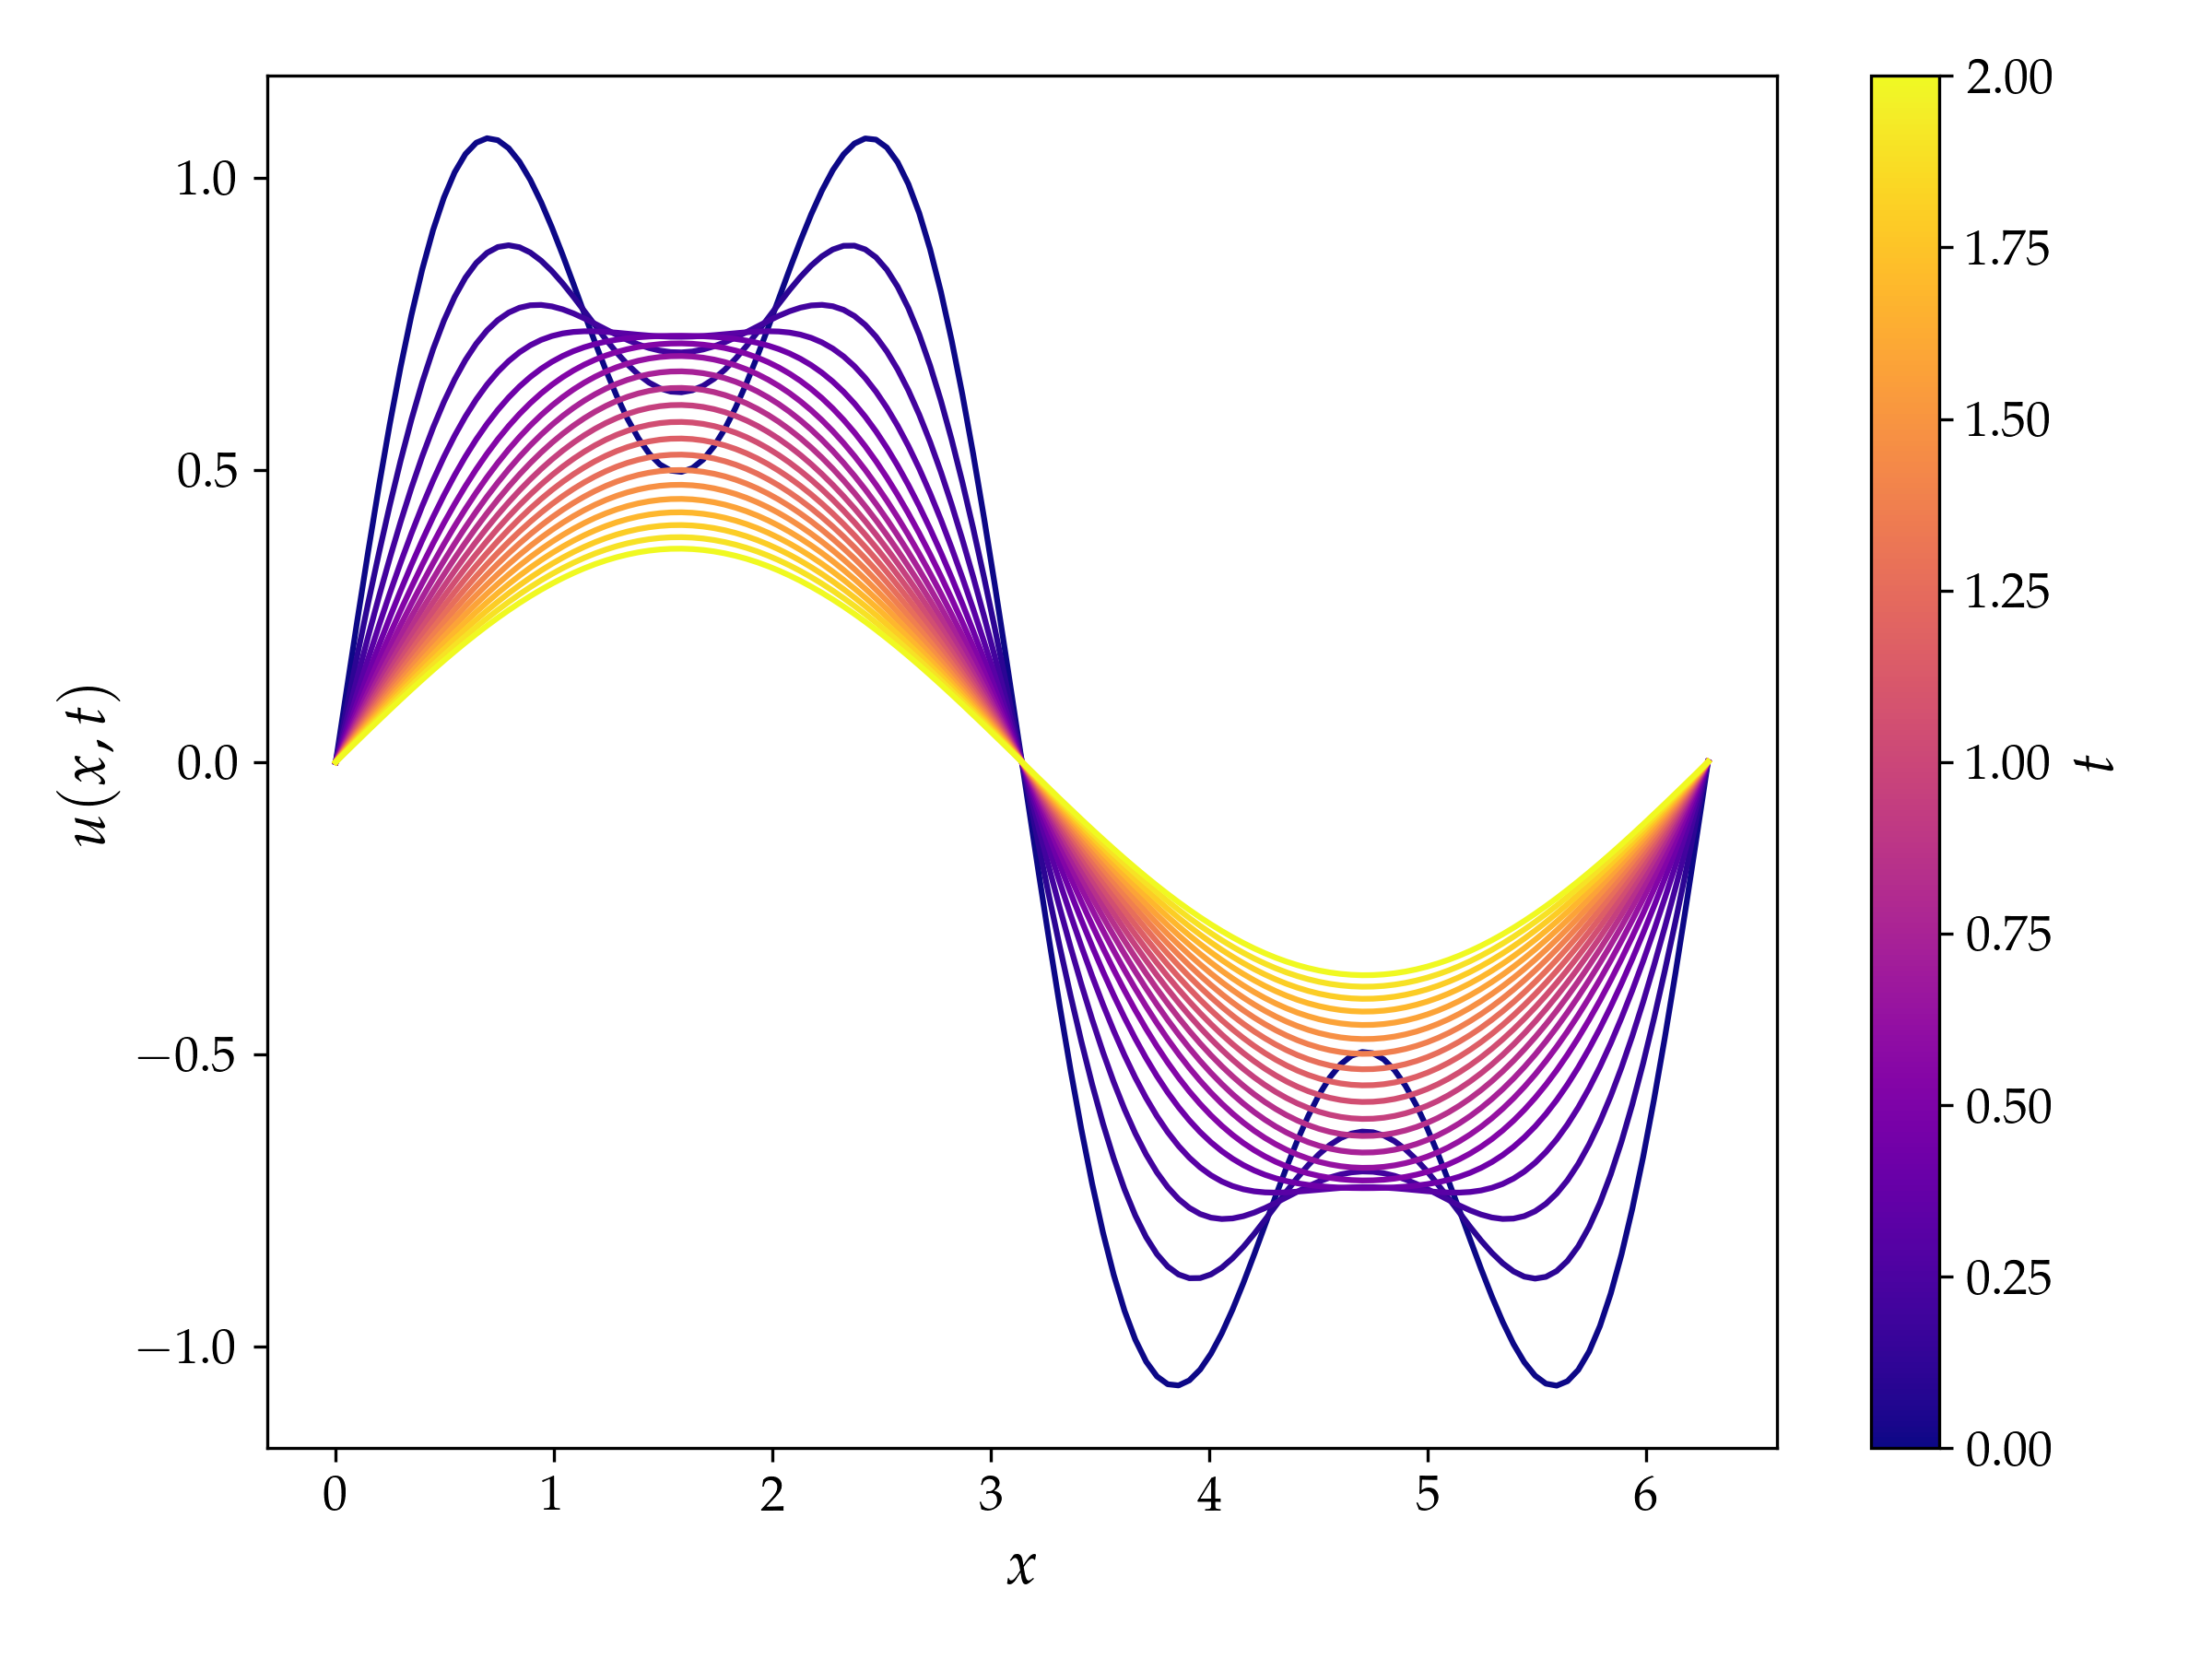
\includegraphics[width=0.8\linewidth]{images/10/heat_sol.png}
    \caption{Variazione del calore in funzione della posizione (asse x) e del tempo (curva di livello con colore assegnato e riportato in legenda).}
    \label{fig: Heat 2d}
\end{figure}

\begin{figure}[H]
    \centering
    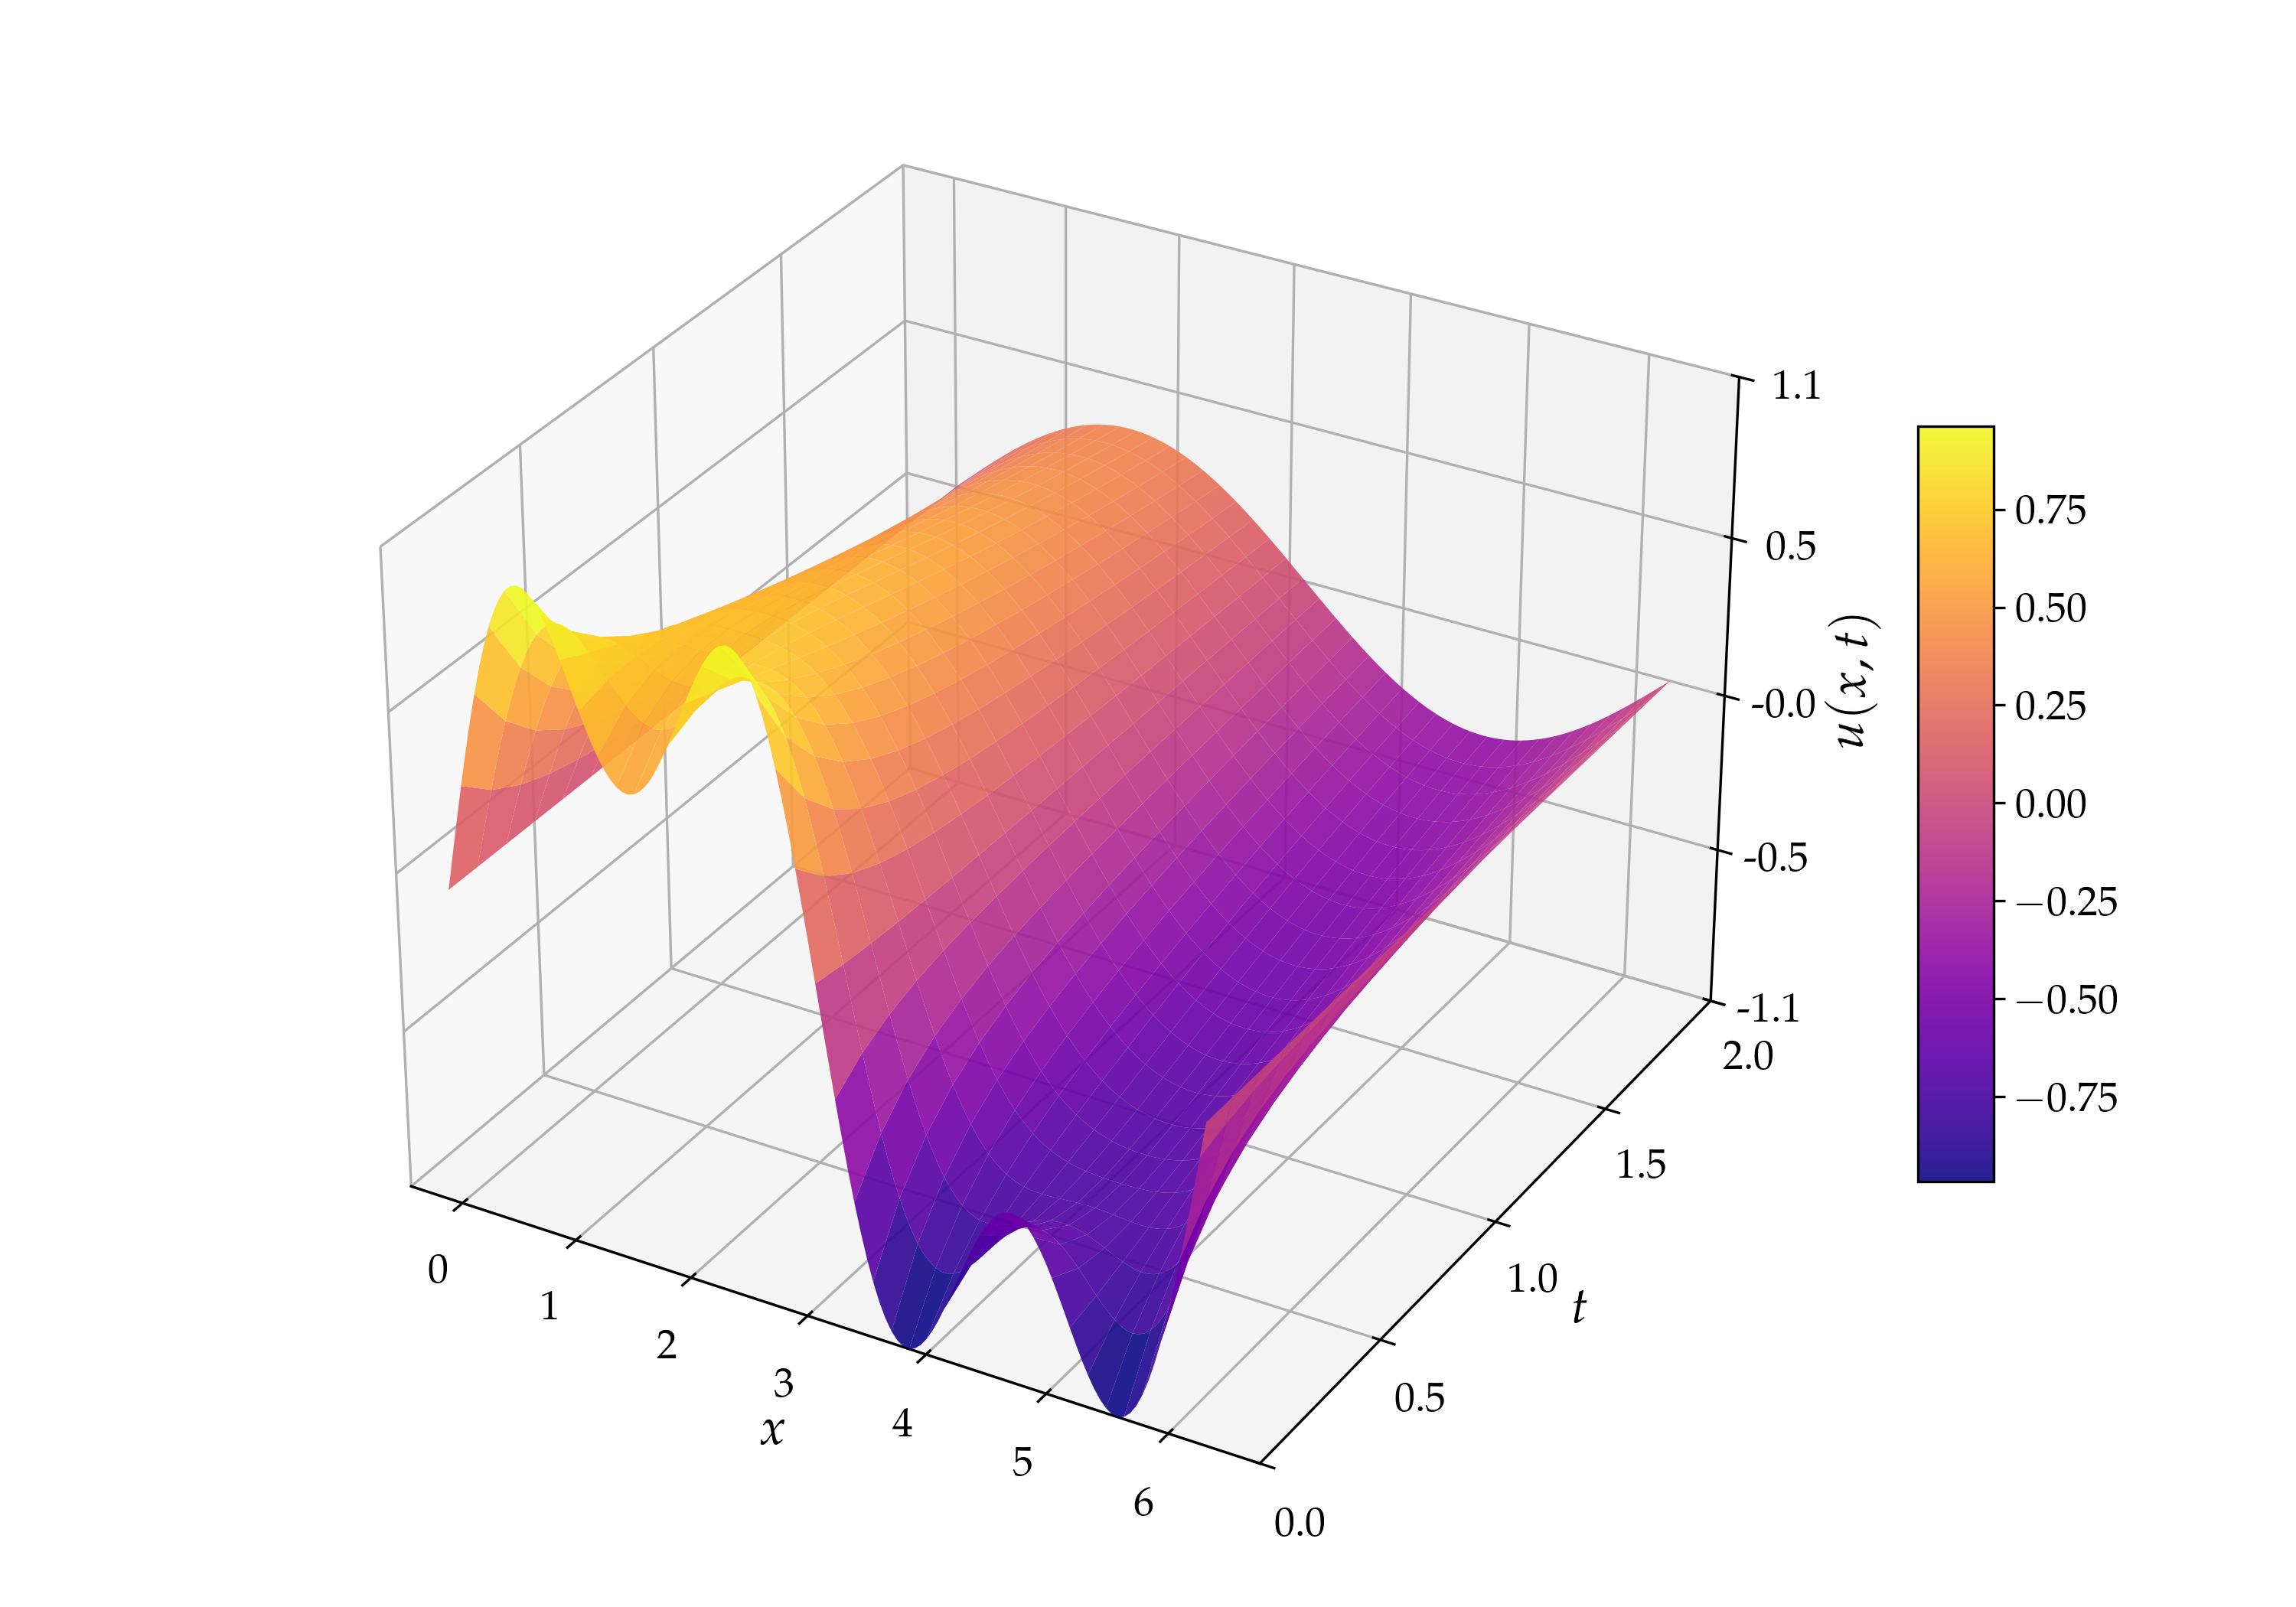
\includegraphics[width=0.8\linewidth]{images/10/heat_sol_3d.png}
    \caption{Variazione del calore in funzione della posizione e tempo con heatmap 3D. Il colore rappresenta il valore della funzione, cioè il calore, come riportato in legenda}
    \label{fig: Heat 3d}
\end{figure}

\newpage







\section{Esercizio 4.5.1}
\subsection{Problem Statement}
Scrivi una funzione che accetti $\{x_i\}$, $\{y_i\}$, $C_{ij}$ e $\{f_a\}$ e restituisca il valore del $\chi^2$ insieme ai parametri del fit e ai loro errori.
Quindi testa la funzione sui dati forniti utilizzando

\begin{equation}
    \frac{F}{(E - M)^2 + \left(\frac{\Gamma}{2}\right)^2}
\end{equation}

\noindent Nota che la forma funzionale non è lineare nei parametri ma una semplice trasformazione può renderla tale! Pertanto dovresti procedere come segue:

\begin{enumerate}
    \item trasforma i dati in modo che la funzione di fit sia lineare nella base monomiale. Produci un grafico dei dati trasformati.
    \item esegui il fit sui dati trasformati e calcola i parametri $F, M, \Gamma$ e il $\chi^2$. È un buon fit?
    \item produci un grafico con i dati trasformati e la funzione di fit.
    \item produci il grafico finale con le seguenti caratteristiche:
    \begin{itemize}
        \item i dati originali (con gli errori)
        \item una linea che rappresenta il valore centrale della funzione di fit
        \item \textit{opzionale}: una banda che rappresenta l'errore della funzione di fit ottenuta propagando gli errori dei parametri del fit.
    \end{itemize}
\end{enumerate}

\subsection{Premessa Teorica}
Se il problema dell'interpolazione è in soprattutto un problema di tipo matematico, in questo contesto vogliamo dare la risoluzione di uno fisico. Partendo da un set di due coordinate, di una forma funzionale che ne descrive la relazione, e degli errori che sono associati al valore sperimentale della funzione, è possibile definire un metodo che esegua un'operazione di grande interesse fisico-sperimentale: in particolare si tratta di verificare il grado di compatibilità dell'osservazione con il modello (test $\chi^2$) e calcolare il valore dei parametri liberi che vengono determinati dall'assunzione del modello come valido.

\medskip
Il set di dati è $\boldsymbol{x}_i$ e $\boldsymbol{y}_i$ rappresenta il valore sperimentale della funzione $f(\boldsymbol{x}_i, \boldsymbol{\alpha}_a)$, dove $\boldsymbol{\alpha}_a$ è il vettore dei parametri liberi, quelli che desideriamo stimare con il fit. Se il numero di punti che usiamo per fittare è $N$ e il numero di parametri $N_A$, allora $i = 0, 1, \dots, N-1$  e $a = 0, 1, \dots ,N_A-1$; 
\begin{itemize}
    \item $N = N_A \implies$ tutti i parametri possono essere fissati esattamente, Fit $\equiv$ Interpolazione.
    \item $N \gg N_A \implies$ 

\end{itemize}

\subsection{Metodi Numerici e Algoritmi}
\subsection{Risultati e Discussione}




\newpage





THE END

% --------------------------------------------------
% INDENTAZIONE CAPITOLI
% --------------------------------------------------
% --------------------------------------------------
% \cleardoublepage 
% \addtocontents{toc}{\bigskip\protect\textbf{\Large LOREM IPSUM}\par\smallskip}
% \addtocontents{toc}{\protect\setcounter{tocdepth}{-2}} 
% \part{\Huge LOREM IPSUM}
% \addtocontents{toc}{\protect\setcounter{tocdepth}{2}} 
% --------------------------------------------------

% \section{Esercizio XXX}
% \subsection{Problem Statement}
% \subsection{Premessa Teorica}
% \subsection{Metodi Numerici e Algoritmi}
% \subsection{Risultati e Discussione}
% \newpage


% \section{Conclusioni}
% % Sintesi dei risultati ottenuti.



% --- Appendice ---


% \newpage
% \appendix
% \section{Appendice: Codici Sorgente e Dati}
% \label{sec: appendice}


% \subsection{Placeholder: Analisi Dati}
% % Inserire qui eventuali script secondari per i grafici.
% \begin{itemize}
%     \item \textbf{Script Plotting:} Descrizione dello script per la generazione dei grafici.
%     \item \textbf{Dati Input:} Struttura dei file di configurazione utilizzati.
% \end{itemize}

\end{document}